% Options for packages loaded elsewhere
\PassOptionsToPackage{unicode}{hyperref}
\PassOptionsToPackage{hyphens}{url}
%
\documentclass[
  donotrepeattitle,doc, 12pt, a4paper,floatsintext]{apa7}

\usepackage{graphicx}
\makeatletter
\def\maxwidth{\ifdim\Gin@nat@width>\linewidth\linewidth\else\Gin@nat@width\fi}
\def\maxheight{\ifdim\Gin@nat@height>\textheight\textheight\else\Gin@nat@height\fi}
\makeatother
% Scale images if necessary, so that they will not overflow the page
% margins by default, and it is still possible to overwrite the defaults
% using explicit options in \includegraphics[width, height, ...]{}
\setkeys{Gin}{width=\maxwidth,height=\maxheight,keepaspectratio}
% Set default figure placement to htbp
\makeatletter
\def\fps@figure{htbp}
\makeatother
\setlength{\emergencystretch}{3em} % prevent overfull lines
\providecommand{\tightlist}{%
  \setlength{\itemsep}{0pt}\setlength{\parskip}{0pt}}
\setcounter{secnumdepth}{5}
% Make \paragraph and \subparagraph free-standing
\ifx\paragraph\undefined\else
  \let\oldparagraph\paragraph
  \renewcommand{\paragraph}[1]{\oldparagraph{#1}\mbox{}}
\fi
\ifx\subparagraph\undefined\else
  \let\oldsubparagraph\subparagraph
  \renewcommand{\subparagraph}[1]{\oldsubparagraph{#1}\mbox{}}
\fi
\newlength{\cslhangindent}
\setlength{\cslhangindent}{1.5em}
\newlength{\csllabelwidth}
\setlength{\csllabelwidth}{3em}
\newlength{\cslentryspacingunit} % times entry-spacing
\setlength{\cslentryspacingunit}{\parskip}
\newenvironment{CSLReferences}[2] % #1 hanging-ident, #2 entry spacing
 {% don't indent paragraphs
  \setlength{\parindent}{0pt}
  % turn on hanging indent if param 1 is 1
  \ifodd #1
  \let\oldpar\par
  \def\par{\hangindent=\cslhangindent\oldpar}
  \fi
  % set entry spacing
  \setlength{\parskip}{#2\cslentryspacingunit}
 }%
 {}
\usepackage{calc}
\newcommand{\CSLBlock}[1]{#1\hfill\break}
\newcommand{\CSLLeftMargin}[1]{\parbox[t]{\csllabelwidth}{#1}}
\newcommand{\CSLRightInline}[1]{\parbox[t]{\linewidth - \csllabelwidth}{#1}\break}
\newcommand{\CSLIndent}[1]{\hspace{\cslhangindent}#1}
\ifLuaTeX
\usepackage[bidi=basic]{babel}
\else
\usepackage[bidi=default]{babel}
\fi
\babelprovide[main,import]{english}
% get rid of language-specific shorthands (see #6817):
\let\LanguageShortHands\languageshorthands
\def\languageshorthands#1{}
% Manuscript styling
\usepackage{upgreek}
\captionsetup{font=singlespacing,justification=justified}

% Table formatting
\usepackage{longtable}
\usepackage{lscape}
% \usepackage[counterclockwise]{rotating}   % Landscape page setup for large tables
\usepackage{multirow}		% Table styling
\usepackage{tabularx}		% Control Column width
\usepackage[flushleft]{threeparttable}	% Allows for three part tables with a specified notes section
\usepackage{threeparttablex}            % Lets threeparttable work with longtable

% Create new environments so endfloat can handle them
% \newenvironment{ltable}
%   {\begin{landscape}\centering\begin{threeparttable}}
%   {\end{threeparttable}\end{landscape}}
\newenvironment{lltable}{\begin{landscape}\centering\begin{ThreePartTable}}{\end{ThreePartTable}\end{landscape}}

% Enables adjusting longtable caption width to table width
% Solution found at http://golatex.de/longtable-mit-caption-so-breit-wie-die-tabelle-t15767.html
\makeatletter
\newcommand\LastLTentrywidth{1em}
\newlength\longtablewidth
\setlength{\longtablewidth}{1in}
\newcommand{\getlongtablewidth}{\begingroup \ifcsname LT@\roman{LT@tables}\endcsname \global\longtablewidth=0pt \renewcommand{\LT@entry}[2]{\global\advance\longtablewidth by ##2\relax\gdef\LastLTentrywidth{##2}}\@nameuse{LT@\roman{LT@tables}} \fi \endgroup}

% \setlength{\parindent}{0.5in}
% \setlength{\parskip}{0pt plus 0pt minus 0pt}

% Overwrite redefinition of paragraph and subparagraph by the default LaTeX template
% See https://github.com/crsh/papaja/issues/292
\makeatletter
\renewcommand{\paragraph}{\@startsection{paragraph}{4}{\parindent}%
  {0\baselineskip \@plus 0.2ex \@minus 0.2ex}%
  {-1em}%
  {\normalfont\normalsize\bfseries\itshape\typesectitle}}

\renewcommand{\subparagraph}[1]{\@startsection{subparagraph}{5}{1em}%
  {0\baselineskip \@plus 0.2ex \@minus 0.2ex}%
  {-\z@\relax}%
  {\normalfont\normalsize\itshape\hspace{\parindent}{#1}\textit{\addperi}}{\relax}}
\makeatother

% \usepackage{etoolbox}
\makeatletter
\patchcmd{\HyOrg@maketitle}
  {\section{\normalfont\normalsize\abstractname}}
  {\section*{\normalfont\normalsize\abstractname}}
  {}{\typeout{Failed to patch abstract.}}
\patchcmd{\HyOrg@maketitle}
  {\section{\protect\normalfont{\@title}}}
  {\section*{\protect\normalfont{\@title}}}
  {}{\typeout{Failed to patch title.}}
\makeatother

\usepackage{xpatch}
\makeatletter
\xapptocmd\appendix
  {\xapptocmd\section
    {\addcontentsline{toc}{section}{\appendixname\ifoneappendix\else~\theappendix\fi\\: #1}}
    {}{\InnerPatchFailed}%
  }
{}{\PatchFailed}
\keywords{keywords\newline\indent Word count: 2004}
\usepackage{lineno}

\linenumbers
\usepackage{csquotes}
\geometry{a4paper, left = 4cm, right = 2.5cm, top = 2cm, bottom = 4cm}


\pagestyle{plain}
\setcounter{tocdepth}{5}
\linespread{1.2}
\usepackage{setspace}
\shorttitle{}
\rhead{DoPL and DOSPERT}
\usepackage{fancyhdr}
\cfoot{\thepage}
\fancyheadoffset[L]{0pt}
\fancyhf{}
\fancyhead[RO,LE]{\small\thepage}
\renewcommand{\headrulewidth}{0pt}
\interfootnotelinepenalty=10000
\newcommand{\HRule}{\rule{\linewidth}{0.25mm}}
\let\cleardoublepage=\clearpage
\usepackage{atbegshi}% http://ctan.org/pkg/atbegshi
\AtBeginDocument{\AtBeginShipoutNext{\AtBeginShipoutDiscard}}
\doublespacing
\ifLuaTeX
  \usepackage{selnolig}  % disable illegal ligatures
\fi
\IfFileExists{bookmark.sty}{\usepackage{bookmark}}{\usepackage{hyperref}}
\IfFileExists{xurl.sty}{\usepackage{xurl}}{} % add URL line breaks if available
\urlstyle{same} % disable monospaced font for URLs
\hypersetup{
  pdftitle={The psychology of risk and power: Power desires and sexual choices. Testing},
  pdfauthor={Ithurburn, Andrew1},
  pdflang={en-EN},
  pdfkeywords={keywords},
  hidelinks,
  pdfcreator={LaTeX via pandoc}}

\title{The psychology of risk and power: Power desires and sexual choices. Testing}
\author{Ithurburn, Andrew\textsuperscript{1}}
\date{}


\shorttitle{RISK AND POWER}

\authornote{

Add complete departmental affiliations for each author here. Each new line herein must be indented, like this line.

Enter author note here.

The authors made the following contributions. Ithurburn, Andrew: .

Correspondence concerning this article should be addressed to Ithurburn, Andrew, 7 George Square, Edinburgh, EH8 9JZ. E-mail: \href{mailto:a.ithurburn@sms.ed.ac.uk}{\nolinkurl{a.ithurburn@sms.ed.ac.uk}}

}

\affiliation{\vspace{0.5cm}\textsuperscript{1} The University of Edinburgh}

\abstract{%
One or two sentences providing a \textbf{basic introduction} to the field, comprehensible to a scientist in any discipline.

Two to three sentences of \textbf{more detailed background}, comprehensible to scientists in related disciplines.

One sentence clearly stating the \textbf{general problem} being addressed by this particular study.

One sentence summarizing the main result (with the words ``\textbf{here we show}'' or their equivalent).

Two or three sentences explaining what the \textbf{main result} reveals in direct comparison to what was thought to be the case previously, or how the main result adds to previous knowledge.

One or two sentences to put the results into a more \textbf{general context}.

Two or three sentences to provide a \textbf{broader perspective}, readily comprehensible to a scientist in any discipline.
}



\begin{document}
\maketitle

\clearpage

\mbox{}\thispagestyle{empty}\clearpage
\setcounter{page}{1}
\thispagestyle{empty}

\begin{center}
\vspace*{10mm}
\rule{\linewidth}{0.25mm}\\
\textbf{\Large The psychology of risk and power: Power desires and sexual choices}\\
\rule{\linewidth}{0.25mm}\\
\vspace*{10mm}
\textbf{Andrew Ithurburn}\\
\begin{figure}[ht]
\begin{center}

\includegraphics[width=!,totalheight=!,scale=0.25]{../Formatting/EdUniCrest.jpg}
\end{center}
\end{figure}
{\setstretch{1.7} 
Doctor of Philosophy\\
\smallskip
\smallskip
THE UNIVERSITY OF EDINBURGH\\
\smallskip
}
\end{center}
\clearpage

\mbox{}\thispagestyle{empty}\clearpage

\newpage

\tableofcontents

\newpage

\hypertarget{chapter-1}{%
\section{Chapter 1:}\label{chapter-1}}

\hypertarget{literature-review}{%
\subsection{Literature Review}\label{literature-review}}

\hypertarget{general-introduction}{%
\subsubsection{General Introduction}\label{general-introduction}}

Research in decision-making is not only concerned with understanding monumental decisions done in a study or saving a life, but equally in more mundane decisions such as understanding choosing what tea to drink in the morning, what clothes to wear that day or whether a couple should have a divorce. Making models of decisions can be difficult given uncertainty is involved along with risk {[}citation{]}. For example, two adult men {[}or a man and a woman{]} that are intending to have sex need to make the decision of whether or not to use a condom. Added uncertainty is involved with the decision-making process. One partner may have multiple sexual partners while the other may have only had one, one partner may have a sexually transmitted infection and might not feel the need or feel comfortable with informing their partner of their status. Consequences of not informing can have dire consequences on both partners.

In 2016, the year of most recent global data collection, there were 376 million necases of the four curable sexually transmitted infections, chlamydia, gonorrheatrichomoniasis, and syphilis (World Health Organization, 2018). The World HealtOrganization {[}WHO{]} further estimates that there are one million new cases of a curablsexually transmitted infection each day. Due to multiple factors, certain minoritpopulations are more at risk for contracting new sexually transmitted infections, e., men who have sex with men and female sex workers (World Health Organization, 2018). Some factors includcertain societal beliefs men who have sex with men might engage in nonrelational sex ``just trying to figure things out it's just a hook up phase'' (Elder et al., 2015) , ambiguous laws concerning the legality of sex work interfering witsafe and available locations for such activity, as well as. There may alsbe some difficulties in their willingness in their activities be it forced by anotheor sheer necessity. For countries like Scotland there have been a reduction ithe amount of new cases of STIs like HIV amongst key populations, however new risks antibiotic resistant gonorrhea, \emph{Neisseria gonorrhoaeae}, have shown a new prevalence in many countries (Ison \& Alexander, 2011).

\hypertarget{who-is-at-risk}{%
\subsubsection{Who is at risk?}\label{who-is-at-risk}}

There is then the arduous task of how to research the topic of sexually transmitted infections and methods of then understanding what is occurring in the individual. There are neurobiological explanations such as certain brain formations occurring that cause individuals to have difficulty understanding the consequences of their actions (Moll et al., 2005; Schaich Borg et al., 2008; Tsoi et al., 2018). There are also more cognitive explanations as well that have shown promising results. For example in the cognitive sub-area of metacognition there is an understanding that there are certain cognitive mechanisms that aid in the individuals ability to regulate their own cognitive understanding of their decisions (C. A. Anderson \& Bushman, 2002; Yeung \& Summerfield, 2012). This self-regulation then contributes to their ability to control whether they act on their baser needs or are able to understand the consequences of what they might or might not engage in (C. A. Anderson \& Bushman, 2002; Crandall et al., 2017). How individuals had reached the information on the effectiveness of certain behavioral changes that reduce the chances of contracting an STI is also in question. For example, research shows that individuals that have a greater understanding of the impact and chances of contracting HIV, actually engage in risky sexual behaviors and therefore increase their chances of contracting the very infection they have more knowledge (D. B. Kirby et al., 2007). Skills based training showed more positive results on practicing safer sex practices. How an individual sees themselves as either a sexual person or person in general is also a factor in how they later may meet an STI (Andersen et al., 1994, 1999; Elder et al., 2015; Gesink et al., 2016). Aggression, in the cognitive sense, also has an impact as well demonstrating a dominance over another person that may cause difficulties in their own ability to make decisions on their sexual health (Malamuth et al., 1996; Williams et al., 2017).

Aggression is one method of exerting control over another individual. Overall, the exertion of control itself denotes a power disparity between parties which varies in effects, methods, and domains. {[}citation{]}. For example, most research has looked at power-over or one person controlling the behavior of another person. This area of research connects the cognitive explanation to behavioral outcomes. Research in power also includes looking at minority populations and aspects of power over to help explain the increased prevalence of certain STIs by discussing and researching certain power dynamics {[}citations{]}. The institutional support of those power dynamics often reflect power based on age, gender, political orientation, sexual orientation and gender identity (C. A. Anderson \& Bushman, 2002; Chiappori \& Molina, 2019; Volpe et al., 2013; Winter, 1988). Investigations of the power structure of a family unit has shown to have some interesting consequences on sexual health depending on the type of parenting style and parental attachment {[}Bugental and Shennum (2002); Chiappori and Molina (2019); Kim and Miller (2020); citations{]}. A new area of research coming out of power and cognition is the phenomenon where an individual will harm themselves in some way to also inflict harm on another. This type of behavior has been researched extensively in the animal kingdom and is known as spiteful behavior in that one brings down their own wellbeing to spite the other person. There would be interesting avenues to research how spiteful thinking may affect an individual in how they choose one course of action over another.
\#\#\# Current Methodology
An interesting aspect of the power dynamics and cognition is the moral aspect of decision-making. Often, sexually transmitted infections and risky sexual behavior are used as examples to discuss moral issues. Methods at understanding these situations and other moral issues are through dilemmas or vignettes where individuals are presented with a short scenario and given the opportunity to choose one outcome over another (Ellemers et al., 2019). A trademark example is the trolley car experiment where there is a runaway trolley car that is going towards five people (Greene, 2001). The decision is thus, allow the trolley to careen towards the five people or you could divert the trolley by pushing and sacrificing a large man for the sake of the other five. This type of dilemma poses an interesting method of understanding how and what the decision maker would choose. The researcher can then change the dilemma on its severity and complexity. There could also be a change in situation and the types of individuals that are at risk. Individual choice tasks investigating risky sexual behaviors and STIs could be furthered with investigating the moral decision-making aspect of those issues.
Current STI research has focused on methods of ways of curbing why individuals act a certain way when presented with a risky sexual situation (D. B. Kirby et al., 2007). Current methods have shown mixed results. In many countries, how people are taught about risk and sex can vary wildly (Unesco, 2015). For example, some countries may have one standard that is a mix of religious and scientific findings of STIs. While others may not even have a formal sexual education program. Some aspects of sexual activity are not even discussed, for example non-heterosexual sex is not always present in education (Ellis \& High, 2004). This becomes problematic in that men who have sex with men tend to be more at risk to contracting an STI than their peers who engage in heterosexual intercourse. There has also been a lot of research in STI rates. Evidence by governments and international health organizations constantly partnering with universities and healthcare providers to collect new incidences of STIs. There might be one way of researching the topic however, it might not look at all the aspects. Some may be more focused on the outcome while ignoring the causes or hypothesized causes of the outcome. Continued research into the understanding of decision-making is important in that understanding the general helps later understanding of the specific.

\hypertarget{risky-sexual-behaviors-and-stis}{%
\subsection{Risky Sexual Behaviors and STIs}\label{risky-sexual-behaviors-and-stis}}

Sexual activity/ability to reproduce being one of the seven characteristics of life can cause health, financial, and/or social dangers (to all participants) through risk and neglect {[}citation{]}. The curability or manageability also plays a factor in how an STI will affect an individual or community. For example, if the treatment is simple and cheap the effect could be minimal. However, if the treatment cost is expensive the drain on multiple resources could be detrimental.

There is a large array of different sexually transmitted infections. Currently, there are eight common types of STIs, chlamydia, gonorrhea, trichomoniasis, genital warts, genital herpes, pubic lice, scabies, and syphilis (Carmona-Gutierrez et al., 2016), chlamydia being the most common. Treatment for these STIs can range from a simple course of antibiotics such as is the case with chlamydia or gonorrhea. Conversely, treatment for syphilis or human immunodeficiency virus {[}HIV{]}, can be increasingly more involved, cause difficulty in daily life, and have higher costs {[}citation{]}. Globally, 37.9 million people are living with HIV {[}104,000 in the United Kingdom{]}, with 1.7 million being under the age of 15 years old (Ison \& Alexander, 2011). The treatment for HIV currently is through antiretroviral medication, which is often a combination of multiple medications to account for the high adaptability of the virus (Costa-Lourenço et al., 2017).

New difficulties appear from the most common treatment strategies. The main strategy for arises given the fluctuating nature of STI treatment and costs. As such, costs for treatments have seen a markable increase with some treatments costing {[}enter average amount{]}. An increasing number of antibiotic resistant gonorrhea is occurring globally, with a recent discovery in Japan with a strain that is resistant to ceftriaxone, the most prescribed antibiotic {[}citations{]}. Two individuals in the United Kingdom recently {[}2019{]} separately tested positive with different strains resistant to not just ceftriaxone but also azithromycin {[}citations{]}. The confirmed cases may seem small however, 10\% of men and half of women do not show visible symptoms when infected with the bacteria. Medical treatment alone has not been the only strides made in STIs around the with strides in acceptances and less persecution for those that have HIV for example. However, while persecution and stereotyping has gone down in recent years, treatments and availability to those treatments have become increasingly more costly.\\
Sexually active individuals can become infected with an STI through various forms. The first and most prominent vector is through risky sexual behaviors, i.e., multiple sexual partners, unknown sexual history of partners/high-risk individuals, and unprotected sex {[}citations{]}. The most common vector is through engaging in unprotected sex. Condoms are the most common and effective method of protection, with spermicides increasing their effectiveness {[}citation{]}. Once infected, the STIs may have detrimental health effects. For example, genital herpes may cause infertility in women and certain types of cancers {[}citations{]}. Infections can also be transmitted to infants during childbirth. If left untreated death is possible for example in the case of syphilis which results in an agonizing death {[}citations{]}. Condoms are still one of the most effective strategies to practice safe sex along with asking partners about their sexual histories.

Even though condoms are the most effective prophylactic, there is still a chance that an individual may contract an STI. Other risky sexual behaviors can increase an individual's susceptibility such as having multiple sexual partners. The age of first sexual intercourse is one of the leading factors that has been associated with increased sexual risk taking and later transmission of STI (de Sanjose et al., 2008; Dickson et al., 1998; Tuoyire et al., 2018). Dickson and colleagues investigated the age at first sexual intercourse and found that women that had their first sexual intercourse before 16 years-old were more likely to report having contracted an STI. In the United Kingdom, age at first heterosexual intercourse has decreased over the last 70 years (Mercer et al., 2013). Mercer and colleagues conducted a longitudinal analysis of age at first sexual intercourse by separating individuals into birth cohorts. Individuals age 65-74 years reported their age at first heterosexual intercourse at 18 years. Every ten years that number has steadily decreased by one with the most recent being 16 years old. Thirty percent of individuals between the ages of 16-24 report have had heterosexual intercourse before the age of sixteen.

Individuals 18-24 years of age are not just having intercourse at earlier ages, they are the group with the highest susceptibility of contracting an STI, amounting for \#\#\#\# of new incidences {[}citation{]}. College students/aged individuals have also increased alcohol consumption which contributes to lowered inhibitions and increased risky sexual behavior. Because many are developing sexually including some living away from home for the first time, they are more likely to engage in sexual experimentation such as multiple sex partners and in some cases may not use protection such as a condom.
Lack of communication has also been shown to influence the likeliness of contracting an STI. Desiderato and Crawford investigated risky sexual behaviors in college students and found that failing to report the number of previous sexual partners and their STI status was common in both men and women (1995). The social stigma of having contracted or being suspected of contracting an STI is one of the most common barriers that inhibits open communication between sexually active individuals (Cunningham et al., 2009). Stigma concerning a positive STI diagnosis can affect not just the physical health of an individual but the psychological health as well. In a series of five experiments, Young and colleagues investigated how the belief of having an STI has an individual's likelihood of getting tested/treatment (2007). They discovered two key points on stigma, others perceive those that have an STI as being less moral and others believe that others will see them as being immoral. This threat of appearing to be immoral may cause the individual to feel as though the mere perception of having an STI is shameful (Cunningham et al., 2009).

The social effects of sexuality in general influence how people see themselves. For gay men in particular there is not just the social stigma that some may have of homosexuality, within the gay community there are some that are expected to be promiscuous or appear to be promiscuous (Elder et al., 2015). In a study based on grounded theory, Elder and colleagues asked gay men all aspects of sexuality to discover and investigate their sexual schemas. A sexual schema is, ``a generalization about the sexual aspects of oneself.'' (Elder et al., 2015, pg. 943). The effects of negative sexual self-schema are also seen in bisexual and straight men and women (Andersen et al., 1994; CYRANOWSKI et al., 1999; Elder et al., 2012, 2015). Having poor sexual self-schema can result in women having issues with sexual desire and an inability of reaching orgasm while in men can result in climaxing too early and erectile dysfunction (CYRANOWSKI et al., 1999; Kilimnik et al., 2018). Long lasting impairments can often lead to more psychological issues.

Individuals that have contracted an STI are also more likely to be ostracized from their immediate community. For example, gay men who contracted HIV in the beginning of the AIDs crisis were often ostracized by society even when they were seeking treatment in the hospital. Nurses would often, for lack of knowledge of transmission of the virus, would often drop medication in front of the patient's door and would rarely physically interact with them {[}citations{]}. This ostracization further compounds the psychological and physical trauma that individuals with HIV already have. As more knowledge of how HIV is transmitted individuals can get more efficient and better treatment. However, ostracization often occurs {[}citations{]}.

\hypertarget{moral-judgment-and-decision-making}{%
\subsection{Moral Judgment and Decision-Making}\label{moral-judgment-and-decision-making}}

Sam has frequent and unprotected sex with multiple partners, resulting in a sexually transmitted infection that causes visible sores on the mouth and hands. On the way to the chemist one day, Sam has an acute heart attack. Bystanders rush to help, but see the sores on Sam's mouth and hands. How would the bystanders react? Would they resuscitate Sam? Would it be morally wrong for them not to risk contracting an unknown disease from Sam, even if it may cost Sam's life? Similar sorts of dilemmas are often used to study moral decision making of various sorts (Clifford et al., 2015). the thought experiment of the trolley dilemma. Research by Haidt and colleagues, compared psychologically normal adults to psychopathic traits and performance on the Moral Foundations Questionnaire {[}MFQ; Graham et al. (2011){]}. Findings included higher psychopathic tendencies were associated with lower likelihood of following justice-based norms, a weak relationship with disgust-based and in-group norms, and finally an increased willingness to violate any type of norms for money (Glenn et al., 2009). The key factor in the Moral Foundations Questionnaire are these moral foundations of which there are five moral domains: harm versus care, fairness versus cheating, loyalty versus betrayal, authority versus subversion, and purity versus degradation (Clifford et al., 2015). Each of these moral domains have a good and bad component compared to the action type.

The MFQ has been extensively used in research on moral decision-making, with common subjects being on political thought {[}citation{]}. In the early studies of moral foundations theory, Haidt investigated the moral foundational differences between individuals that lean either politically liberal or conservative. Of the five moral domains, differences appeared in the likelihood of how either conservatism or liberalism affects the likelihood of individuals to endorse each domain. For example, liberalism suggests protecting the individual from harm by the society, especially if they are a member of a minority group. Conversely, conservatism, namely religious conservatism suggests a propensity for sanctity and purity, along with respecting authority and following the societal moral codes {[}citations{]}. Emotional valence is often the best predictors of moral judgments {[}citation{]}. The more emotional valence the faster the response time the decision-maker decides and the more staunchly held they are to their decision. Interestingly, participants would be unable to express or support the decisions that they made. Often, participants would downplay their decisions by laughing or stuttering (Haidt, 2001). Additionally, as their emotional valence of the decision is higher, people are consistently holding on to their judgments regardless if they were able to support their judgements when asked or not. It then makes sense why some individuals are more politically intransigent given their deeply held moral codes.

Politically held beliefs are often emotionally laden (G. Marcus, 2000). Accordingly, moral foundations theory postulates that there is a good versus bad in the moral domains. When participants are asked to respond to statements that are only offensive but were not harming anyone, participants had issues supporting whether the statement was good or bad. For example, when participants were given a story of cleaning the toilet with the national flag, participants would respond that it is bad and said that they just knew that it was wrong {[}citation{]}. Often when individuals violate the moral rules of ``cleaning the toilet with the national flag'' violators will be judged as immoral and sometimes punished for their actions {[}citations{]}. Intuitively the participants responded that the actions were morally were obviously morally wrong. Requiring little to no explanation as to whAn interesting facet of moral judgment is how individuals react to moral decisions when they are reminded of their own mortality (Greenberg et al., 1990; Rosenblatt et al., 1989). Reminding individuals of their mortality causes them, according to terror management theory, to want to push away from the thought of their eventual death. To do this people often cling to their deeply held cultural beliefs to remove their thoughts from reality (Greenberg et al., 1990). In the first of a series of experiments Rosenblatt and colleagues found that participants that were reminded of their mortality judged prostitutes more harshly, more so if the participants already had negative opinions on prostitution. This was also seen conversely with heroes that follow the cultural norms. Those participants advocated for a larger reward for those individuals (Rosenblatt et al., 1989). The already held opinions were further investigated to where Christians were asked to report their impressions of Christian and Jewish individuals after mortality became salient. Those that were a member of the in-group, Christian, were more likely to be regarded as more positive than their out-group counterparts, Jewish individuals (Greenberg et al., 1990). In-group bias is an oft studied concept in psychological research. Mortality salience and moral violations tend to increase the strength of the in-group bias and then moral judgement and condemnation {[}citation{]}.

When a person does a negative action, the reason for the action is often judged and assumed. An action is commonly seen as being intentional when the individual actively does the action directly. However, intentionality becomes problematic participants have already had negative evaluations of the individual. In an experiment where participants were asked to judge the culpability of an airline passenger that was forced by high-jackers to kill another passenger, the high-jackers were the external force forcing the passenger to commit murder. However, when the participants were told that the passenger already wanted to kill that passenger before the hijacking was occurring, they were judged as more culpable. With or without the internal motivation of wanting to already kill the other passenger, the resulting death still occurs. When participants were given a, less vivid, story of a manager that was only mistreated a black employee and another story of a non-bigoted manager that was mistreating all of their employees, participants judged the bigoted manager more negatively. Even though there were differences in those affected between the managers, participants already held a negative opinion for those that hold bigoted views, and thus judged the bigoted manager more severely {[}citation{]}.

Research in attributional blame continued with an experiment investigating passengers on a sinking boat (Uhlmann et al., 2013). Participants were given a story where there were several individuals on a sinking lifeboat. There were too many people in the boat and the only course of action given was that some of the passengers had to be thrown overboard. In the utilitarian perspective, used for this example, the morally correct judgment was a few must be sacrificed for the safety of the larger group {[}citation{]}. However, the participants often judged the surviving passengers as acting selfishly. Thus, they were seeing the passengers as immoral.

When individuals commit a moral violation, as would be the case for the surviving passengers, it is not only important to investigate how others would judge and react but also how the individual reacts to their own action (Tangney et al., 2006). Emotional reactions occur when someone does a behavioral action, or they expect a behavioral action to follow. An interesting aspect of emotional reactions are emotional reactions tied to moral judgment. When an individual violates a moral norm, they often feel a personal feeling of shame or guilt which are two of the most commonly studied of these self-evaluative emotions (Tangney et al., 2006). There is an inherent difference between these two emotions, shame is inferred as being negative feelings of oneself that has a public display, while guilt is similar sans the public display (Tangney et al., 1996). Individuals who violate the community's customs on purity often feel a sense of shame. While guilt is commonly felt with a violation of community {[}citations{]}. People with STIs are often left feeling shame from their suspected purity violation and thus are often stigmatized for their behavior and punished in some form by the community. This can lead, as discussed in the previous section, to increasing their sense of isolation and negative self-worth. How the moral violators react to their shame or guilt is dependent on whether they experience the former or the latter.
There are often attempts to amend the situation when individuals have violated moral norms. Depending on the self-evaluative emotion that is being felt, people will make amends to try to change the situation or they may hide it (Tangney et al., 1996). Guilt is the former and shame is the latter. In most cases individuals that are feeling shame will attempt to ignore their moral violation where they will deny or evade the situation that is causing them shame. Conversely, people with guilt are often motivated by those negative feelings to fix the situation that caused them to feel the guilt. Guilt is often feeling negativity towards a specific action while feeling ashamed or shame is usually a reflection of the entire self {[}citations{]}. Thus, in relation to how to repair the guilt inducing act, it would appear to be more manageable if the inducing situation was a singular event rather than a feeling of the entire self. Participants that were prompted to feel shame were less likely to express empathy for someone with a disability (Marschall, 1998 as cited in Tangney et al., 2006). When people feel a sense of shame, they self-evaluate and reflect on themselves. This hinders the empathy process that would require them to focus their attention on the emotions of another person.

Barnett and Mann investigated sexual offenders to understand how feelings of empathy are blocked for their victim at time of the offense (2013). In empathy research, emotions cannot only just be inferred by the situation but be ``felt'' to be classified as expressed empathy. Earlier research looking at empathy by sexual offenders has not shown them as being unempathetic. However, Barnett and Mann contend that sexual offenders may have a disruption in seeing distress in their victim. The offender may then believe and assert that their victim deserves the distress that they are experiencing and have a cascading effect where they may be powerful and enjoy the distress of the victim (Barnett \& Mann, 2013).

\hypertarget{power}{%
\subsection{Power}\label{power}}

A common denominator in research on the dark personality and moral judgment is the influence of power. To define power, one would have to first define the actor and the recipient of the power. Therefore, there is either power-over, power-to, and power-with. Each aspect has their own different consequences {[}citation{]}. Power-over is when there is one individual, the one with power, which wields control over a subordinate individual {[}citation{]}. Power-to is when an individual of privilege uses their status and power to control and enact a certain consequence {[}citation{]}. Finally, power-with is an interesting concept where a person of power uses their own power to lift or elevate someone without power to a power position {[}citation{]}. This is often seen in community projects where someone in power goes into a troubled community and facilitates the situation so that those that have less power can have their voices be heard. Power also has various sources each with their own complex consequences: institutional, cultural, gender, age, ethnicity, orientation, and gender-identity {[}citations{]}. Some sources of power compound on one another to increase the level of power over other singular sources of power. For example, in many areas of the world a straight white cisgender man would hold the most power relative to other individuals.

Power influences relationships be it romantic or familial, work, academics, including each of their derivatives. The three variations of power have various influences on each of the areas of life. Power is neither good nor bad, it is how the power is used that makes it either good or bad {[}citation{]}. Power and power structures are often in the media. Often when there is a military coup in a far-off country, individuals discuss power-over. When a humanitarian goes into an impoverished community to help their voices heard, power-with is discussed. As with the previous example, when a legislator uses their influence to pass a law, that legislator uses power-to.

Early discussions of power descended from Greek and Roman political philosophy (Aristotle, 1984). Greek Philosopher, Plato's brothers Glaucon and Adeimantus discuss the viability or requirement of citizens being just and lawful if they are able to escape conviction because of some social power or fortune (Aristotle, 1984). Aristotle continued the discussion by posing the questions, ``There is also doubt as to what is to be the supreme power in the state: Is it the multitude? Or the wealthy? Or the good?\ldots{}'' (Aristotle, 1984). Power discussions such as that by Aristotle point to what is the source of someone's power. Does the power come from the majority? Does it come from money? Does it come from those that are just? Each source of power has different effects on those that are governed by those with that power. Polybius of Greece discussed how a constitution should be created and power should be delineated. Polybius power should be split between multiple groups, each with a different form of power and distinct genre to wield that power {[}citation{]}. Power continued to be discussed well beyond the Greek philosophers and continued by political researchers and philosophers. Discussions of power soon developed into research on how it influences at the community level.

Sociologists, following many of the philosophical thought experiments previous and current to the time, began to research power. Sociologists soon developed the area of research in social power, where political power was a subset. According to Bierstadt, power is always successful, whenever it fails then it is no longer power {[}1950{]}. Sociologists asserted that power be conceived of as a force, something that is applied to control a situation. Power can also be conceived of as more passive authority. There are three sources of power: number of people, social organization, and resources. From that individuals that are the class or group or have the most resources that are in need are those that will have the most power. Resources need not be physical objects they can also be more psychological such as skills or knowledge. From history there are many examples where power becomes toxic and the leader becomes the oppressor. Be it Mao Ze Dong, Stalin, Lenin, or Hitler. The question then becomes what causes the powerful to become oppressors? In some cases, those that are in power are trying to do good for the community, restrictive from the example.

Recently, issues and abuses of power have become much of the forefront of news due to the explosion caused by the me-too movement {[}citation{]}. The me-too movement was first coined by activist and sexual harassment survivor Tarana Burke. A decade after she disclosed her sexual assault, the me-too movement and the abuse of power dominated the new cycle with accusations against film producer Harvey Weinstein {[}citation{]}. Weinstein was known for doing philanthropic initiatives during his career by using his influence and money to aid the certain initiatives that he had chosen. However, soon news of his sexual assault accusations and threats became news. Soon multiple women came forward accusing Weinstein of assaulting them as well and using his power over them to intimidate and silence them {[}citation{]}. This exemplifies how resources and position aid in individuals become powerful. Weinstein had the resources and the authority to abuse his power with many of his peers knowing what he was doing {[}citation{]}.

In psychology, it was originally conceived that power corrupted individuals exemplified by the Stanford prison experiment where ``regular'' individuals were instructed to play the prison guards of a simulated prison. Similar individuals were instructed to portray the prisoners {[}citation{]}. Zimbardo, the lead researcher for the experiment, soon noted that the individuals that portrayed the prison guards became aggressive with the prisoners. They verbally and physically assault them. The experiment was halted to stop any more damage from occurring. News spread of the results of the experiment and power was seen as causing or influencing the ``prison guards'' to become aggressive and abuse towards the ``prisoners.'' However, the nature of the participants became into question {[}citation{]}. Later researchers noted that there could have been a self-selection bias of the participants. The experiment was advertised such that the prison experiment was known to the participant. This would then cause individuals to self-select into the group which could possibly skew the results given that the participants may have had authoritarian tendencies and the experiment and added power may have given the opportunity for the participants to express their authoritarian tendencies already present {[}citation{]}. Similar explanations have occurred in politics.

Throughout political history individuals that have reached powerful positions on multiple occasions have given some powerful people the outlet to express their prejudiced and problematic beliefs {[}citation{]}. Fear of communist infiltration in the United States caused many fears and blacklisting was a frequent practice. Joseph McCarthy, a Wisconsin senator, would soon use his power as a legislator/senator {[}citation{]}. McCarthy would call individuals to the front of the House Un-American Activities Committee because they were suspected of being spies for the Soviet Union. McCarthy and the committee used strong arm tactics and would often threaten individuals brought in front of the committee. Many individuals brought forward often had their lives irrevocably changed {[}citation{]}. Soon Senator Margaret Chase Smith and six others condemned McCarthy for his actions and tactics. McCarthy was soon censured, and the House Un-American Activities Committee was disbanded. The political issue of power being used as an outlet for prejudiced and authoritarianism became apparent recently after the 2016 United States Presidential Election {[}citation{]}. Donald Trump's political exploits would soon highlight his past and present use of power and his unethical dealings. Often Donald Trump would use his power for personal gain and to express his prejudicial and racist beliefs. Examples range from in the 1990's Donald Trump advocated for the Central Park Five, five African-American men accused of raping and murdering a young White woman in Central Park, to be put to death {[}citation{]}. However, DNA evidence exonerated on the men of the crime {[}citation{]}. Recently, Donald Trump on the campaign trail accused Mexico of sending individuals across the border that were rapists and drug dealers. However, there was no physical proof of the case and became a common trope used by Donald Trump supporters. Because of the misuse of power and authority, there have been increased hate crimes towards Mexican Americans and African Americans {[}citation{]}. The Southern Poverty Law Center, an organization that records the number of hate groups currently active in the United States has documented a clear increase in the number of active hate groups after the 2016 election {[}citation{]}. The supporters feel a sense of validation for their own beliefs and opinions which they feel allows them some power in and of itself. This then poses an interesting question in power research in psychology. What are the correlates of the power complex? What are the consequences of power? How does a power imbalance affect relationships? The list of questions is vast and varied.

Power imbalances in relationships can have negative effects spanning the entirety of an individual's life, be it emotionally, physically, psychologically, and socially {[}citation{]}. Dr.~Helene Papanek, director of the Alfred Adler institute, a sub-clinic of the Alfred Adler Mental Hygiene Clinic, discussed at a meeting of the Association of Humanistic Psychology, multiple cases of controlling and power disturbances in personal relationships. A relational example was presented where a father, Mr.~A had complete control over his wife and daughter. Controlling when they should be home and where they should go. Mr.~A even controlled the frequency and positions of sex (Papanek, 1972). Power-over someone can also manifest feelings of low self-worth and destructive behaviors. For example, Ms.~C was a young mother of a child born out of wedlock. She was abandoned by her parents and the father of her child. She was constantly controlled by her mother and their disdain for her child out of wedlock. Soon she developed panic attacks but also a sense of superiority over others as a defense mechanism. Dr.~Papanek noted that Ms.~C developed and lived a life of spiteful behaviors one after the other.

The behaviors of Ms.~C and Mr.~A are not the only examples of individuals having power over another person or being subjected to the power over them. Power-over has occurred throughout human history and is ingrained in all cultures {[}citation{]}. Institutional power-over is quite common cross-culturally. Contraception and control over one's own reproductive system is a prescient debate globally {[}citation{]}. In 1960 and 1963 Enovid was approved for use in the United States and United Kingdom respectively {[}citation{]}. Doses for contraception early on were often high and news of multiple deaths was reported widely. Cases were brought forward to control the use of contraception. The Roman Catholic Church's stance on hormonal contraception shifted from permission to outlawing anything that would be believed as stopping the ability to propagate {[}citation{]}. Interestingly in 1989 researchers working for Pfizer in the United Kingdom were researching a new drug that would aid in treating heart conditions {[}citations{]}. The researchers soon discovered sildenafil also could treat erectile dysfunction. Ten years later, sildenafil, brand name Viagra, would be patented and approved for use for the primary treatment for erectile dysfunction {[}citation{]}. The same individuals that were trying to reduce the use of female contraception were not trying to do the same for Viagra. The Japanese government and officials had similar attempts to quell the use of female contraception while not doing the same for erectile dysfunction treatments {[}citation{]}.\\
The Council on Foreign Relations {[}CFR{]} a non-profit that specializes in the United States and international affairs, conducts an international index on women's workplace equality by rating each country on factors: accessing institutions, getting a job, going to court, protecting women from violence etc. {[}citation{]}. Scores range from 0 to 100 where 100 is near total equality in all areas. Of 189 countries on the list only 9 scores over 90\% in the ranking. One hundred and thirty-eight score below 75 with Yemen having the lowest score of 24.5. Including those that intersect with other minorities have even less power like women of color and trans individuals {[}citation{]}. Women having less power than their male counterparts can have multiple negative outcomes such as continued and sustained sexual aggression, low self-esteem, financial insecurity, lack of freedom of movement, lack of freedom of thought, and in some extreme cases even death {[}citations{]}. Cultural relativism creates a difficulty in cultures that have opposing views on the rights and how to navigate that can in and of itself reflect institutional power imbalances.

Power imbalances can create a dissociative state where those with less power are seen as more of an object than a person (Gwinn et al., 2013; Haslam \& Loughnan, 2014; Lammers \& Stapel, 2011; Smith, 2016). While others with more power may see those with less as be less human, some individuals attribute the dehumanization to themselves as well and self-dehumanize (Bastian et al., 2013; Bastian et al., 2012; Bastian \& Haslam, 2010; Kouchaki et al., 2018). Effects of prolonged dehumanization by those with more power often, unchecked and under constant pressure, can lead some individuals to believe what the powerholders say is true. The question remains, why do people in power begin to dehumanize those with less power? Commonly when an individual harms another usually there is some perspective taking by the harmer. However, to dehumanize the other person it lessens the sense of empathy that one would normally feel thus allowing for more damage and harm to be committed {[}citations{]}. ``With great power comes great responsibility'' often quoted by Uncle Ben in the Spider-Man comic books, yet has its possible historical foundations in the French National Convention in 1793, leads credence to the wane and flow of the effects of power (Nationale (Paris), 1793). Those in power make decisions for those for which they are leaders. As is the case with every decision there is a reaction to the decision. Sometimes those effects are negative and those with less power may be harmed in the process. Dehumanization of those in less power acts as a defense mechanism to continue making life changing decisions.

Often dehumanization is left to more extreme occasions such as war, infrahumanization, where ascriptions of nonhuman qualities are more subtle and not as extreme (Haslam \& Loughnan, 2014). Research in dehumanization/infrahumanization by Gwinn and colleagues used game theory and university students to simulate power differentials (2013). In their research, they found that once individuals began to gain power, they would ascribe fewer humanlike personality traits than those with less power ascribing traits to the powerful. Interestingly, there is a reciprocal relationship between self-dehumanization and immoral behavior (Kouchaki et al., 2018). When individuals would commit an immoral behavior, they would afterwards often feel less human, which in turn has them act more immoral.

\hypertarget{cognition}{%
\subsection{Cognition}\label{cognition}}

When deciding, the decisions are not subject to a vacuum. Every decision that is made is contingent on the prior understanding and knowledge of the situation and the possible outcomes of those decisions. The woman choosing one tie over another or the little boy choosing one doll to play with is contingent on the knowledge that they both separately have gained in their lives so far. It could be said that the time at which an infant is first learning about the world is when individual decisions are made by instinct without gained knowledge. When the infant ages and acquires more memories from the environment, it will begin to use those memories in making future decisions.

The first step at acquiring new knowledge is interacting with the environment. One explanation that has been garnering more cognitive and biological attention is from Dr.~Nelson Cowan's integrated working memory model (Cowan, 1999). In the integrated working memory model there are four key areas in attaining new information: {[}1{]} a brief sensory store, {[}2{]} a long term store, {[}3{]} the focus of attention, {[}4{]} and the central executive. Each key area has a separate function{[}s{]} that allows for new information to be ``judged'' against the existing information. The information that is then held temporarily in a sensory store to where it is then sent to the long term store to be ``directed'' by the central executive which is a metacognitive process that controls and directs where attention should be placed on the incoming information. There is then a controlled more conscious action or an automatic action based on the type of incoming information. Information that is automatic usually is considered habituated to the memory system and is therefore not a novel stimulus. More focus is given to information/stimuli that is more novel. In the integrated working memory model information that is incoming in the brain is often ``filtered'' through a lens that is understandable to the individual, novel stimuli. From here the information is then encoded and stored in long-term memory for reactivation by new stimuli.

The integrated working memory model is similar in thought to how individuals make decisions based on the laws and customs of a society. Johnathan is a normal member of his community. They participate in a common game in the park with some friends. Johnathan says an inappropriate joke to one of their friends. The others overhear and judge, automatically, the content of the joke to the governed norms of the community. Because this joke is outside the common norms of the community, the others see Johnathan as violating their moral code. Johnathan's friends would then automatically analyze the joke against existing information and attend to the key features. Like how the central executive guides and directs attention to the new novel stimuli, the inappropriate joke. Interesting research has been done with morality and metacognition.

Common to research in metacognition and moral reasoning is theory of mind. A theory of mind is the ability for an individual to attribute or recognize the inner workings of the mind and differentiate those from the self and others {[}citation{]}. Research in theory of mind has contributed to our understanding of autism, schizophrenia, and traumatic brain injury (Byom \& Mutlu, 2013). An individual with deficits of theory of mind would for example be unable to attribute signs of happiness on other people, such as a smile or a frown {[}citation{]}. In the case of Johnathan, if they had a theory of mind deficits, they would be unable or have difficulty in noticing the dissatisfaction of their joke. Research using theory of mind to investigate social situations such as the example with Jonathan helps psychologists get a better understanding of how moral judgement works and is affected by deficits in the cognitive system.

As discussed thus far, cognitively, each component contributes and affects the individual in a multitude of ways. As previously discussed in the section on risky sexual behaviors, how the individual sees themselves and how they believe others see them is exceptionally important to their overall cognitive health. These sexual schemas that each of us create about ourselves is influenced by daily interactions and prior history, whether sexual. Outside of how the sexual schema individuals create about themselves affects their later sexual health, it can change how they see and interact with the world around them.

The prior knowledge that individuals have can have a negative effect on their ability to gain and hold new information. Those with lower prior knowledge of a given technology often have difficulty in reconstructing the information of a new product compared to those that have less prior knowledge {[}Wood \& Lynch, 2002{]}. When people are presented with new information, a new technology, encoding of the new information takes place. As that occurs, prior information of the technology is retrieved, and an inference is made on subsequent information by comparing the new and old information. This affects the ability to encode the new information ``correctly'' and can disrupt later retrieval of the former. Similar effects are seen when investigating motivational forces. Individuals with prior knowledge may also have an overconfidence of the information that they already have and are not as motivated to attend to the information they are learning.

Extending the research on prior knowledge and new technology, prior knowledge and complacency has also been seen with contracting an STI, a virus, or chances of getting pregnant {[}citations{]}. The decisional factors that occur cognitively to choose safe sex practices is complex and subject to frequent change. Many people that are confronted with decisions, such as the mundane choice of what shoes to wear, base their decisions from using a variety of cognitive methods. Often, the choice to wear a condom or other safe sex practices is through a risk heuristic of contracting or transmitting a sexually transmitted infection. With decisions based on issues of purity, such as sex, one heuristic that is commonly employed is the affect heuristic. The affect heuristic in judgements of risk is where the thought or priming of a specific word triggers a quick emotional response to that stimuli word (Finucane et al., 2000). When presented with words that are physically harmful such as cigarettes or pesticides, participants rated the words as too risky and reported negative feelings concerning those stimulus words. Affective considerations of high-risk situations are often put into perspective with individuals in risky situations.

An artifact of how issues such as HIV, Human Immunodeficiency Virus, discussed in the media and the community that it affects creates a cognitive problem with individuals judging the likelihood of catching the virus, especially women. In the media it is often discussed how men who have sex with men are the main individuals catching and spreading HIV. While HIV still affects the LGBTQ+ community, the discussion around susceptibility affects other individuals outside of the LGBTQ+ community negatively as well. Women, for example, have a genetically higher susceptibility to the virus {[}citation{]}. That being so, often due to unintended ignorance to their chances are one of the leading groups contracting new cases of HIV {[}citation{]}. Downlow culture as well increases the chances of contracting the virus. Amongst some men that do not wish to acknowledge their own homosexuality will choose to forgo the condom, implies a premeditation, and do not necessarily believe they will contract the virus {[}citation{]}. Both examples are contributed by the representation of HIV in the media and the current zeitgeist.

Common in all decisions is the difficulty and uncomfortability between different decisions and opposing situations, is cognitive dissonance (Festinger, 1957). An interesting cognitive dissonant series of thoughts that some males have is when choosing to wear a condom. Often, there will be the cognition of not wanting to contract an STI, but also believing that condoms are uncomfortable (MacPhail \& Campbell, 2001). In addition to believing they are uncomfortable there is an interesting cultural belief amongst some young men that wearing a condom makes them less of a man (Pleck et al., 1993; Vincent et al., 2016). To some the main decisional factor in whether to wear a condom is not contracting an STI or getting pregnant {[}citation{]}. While, as noted with perceptions on condoms, often comfort and how others will see them is the main factor. Sexually active or those thinking to become sexually active often get their opinions on sexual activity and safety practices from their peers. Often, the opinions of peers are more influential than those of the parent{[}s{]}. Interestingly, some men believe that due to the cultural cognition around contraception, discussions and decisions of contraception is a female decision (Castro-Vázquez, 2000).

\hypertarget{aggression-and-cognition}{%
\subsubsection{Aggression and Cognition}\label{aggression-and-cognition}}

Connected to spitefulness, moral judgment, and cognition is human aggression. Traditionally, aggression is differentiated between the outcome or motivation of the incident. Aggression as it is operationally defined is behavior that is committed by the actor to another with the intent to harm the other (C. A. Anderson \& Bushman, 2002). This is then further differentiated to violence where violence is the intent to cause severe harm such as death. From aggression research and moral judgment, cognitive neoassociation theory {[}CNT{]} was beginning to become tantamount in research on aggressive behavior.

In CNT, similar to the study of disgust association where some research suggests that inducing the disgust response to smell causes individuals to become more conservative against breaking moral norms (Eskine et al., 2011; Horberg et al., 2009; Laakasuo et al., 2017; Tybur et al., 2009). Important to the present discussion on sexual judgment, research by Laakasuo and colleagues suggest that disgust is only predictive of sexual disgust (2017). From CNT, Anderson and Bushman developed the General Aggression Model {[}GAM{]} is a theoretical outline that combines multiple smaller domain specific theories on aggression like CNT (2002). The GAM has processes: inputs, routes, and outcomes of a social situation. The inputs separate into a person and situation centered inputs. The individual then has an internal examination of the person or situation, cognitions like affective processes, availability heuristics, theory of mind evaluations, scripts and schemata {[}Barnett and Mann (2013); Kahneman and Tversky (1972); scripts and schemata citation{]}. Appraisal and a decision process are the last step in the GAM, where the individual evaluates the situation based on the inputs and routes. Anderson and Bushman contend that there are two types of outcomes, thoughtful and impulsive actions. Like the affective heuristic, the impulsive action is often fast and does not require as much deliberation. While the thoughtful action requires more time and evaluation of all the possible outcomes.

Scripts and schemata are key components of the GAM. Schema, more broadly than sexual schema, are cognitive compositions or structures that represent objects or ideas interconnected by their features (DiMaggio, 1997). Multiple representations of schema and stereotypical event sequences are labelled as scripts (Abelson, 1981). A classic example of a cognitive script is events surrounding reading the menu at a restaurant (Abelson, 1981). An individual is at a restaurant and needs to order from the menu. However, they lost their reading glasses. As Abelson contends, the reader must infer what is needed in reading a menu, what occurs at a restaurant, and so on. The automatic process of schematic activation begins with certain key features of an object or event being noticed by the individual. For example, recognizing a tree one of the first features that are noticed that distinguishes a tree are the leaves. From the leaves, the bark is activated, and so on making up the concept of a tree.

Often aggression and discrimination can be understood through the schematic model. Media and social representations of individuals, especially men of color, have often made assumptions and portrayed them as violent and criminals. Currently a majority of US adults in a recent Pew Research Center poll report that race relations are currently worse, Black Americans and people of color in general report more cases of discrimination, and a majority say Black Americans in particular are treated unfairly by the police (Pew Research Center, 2019). Aggression or discrimination is often the result of associating one group with negative connotations. For example, in the case of those that believe Black Americans are criminals they have through cognitive associations have related the schematic concept of criminal with the features/schema of what they believe is a Black American. The discrimination and aggression then occur through the GAM processes with negative actions being the outcome.

Pertinent after the advent of the me-too movement, see section 3, issues of how these power over views of women, especially women of color and trans women of color, become learned and develop in sexual aggression. Sexual aggression in and of itself is a subgroup of aggression where the intent to harm is sexual in nature (C. A. Anderson \& Bushman, 2002; Malamuth et al., 1995). Many of the targets of sexual aggression are women of color and trans women of color {[}citations{]}. In the reported cases men are often the perpetrators of the crimes (C. A. Anderson \& Bushman, 2002). The aggression itself appears to be domain specific to one gender, women. Often, acts of sexual aggression are verbal in nature, such as asking repeatedly for sex or threatening to break up with them (Testa et al., 2015). When individuals gain power they may aggress more over those that have less power, which may pay head to the continued sexual aggression and sexual violence against women of color and trans women of color for whom have historically low levels of power {[}citations{]}.

Recent research by Garnett and Mann investigate the cognitive and empathetical processes of those that commit a sexual aggression or sexual violence, labeled as sexual offending (2013). Common to research on sexual offenses, research contends that those that do offend do so with a lack of empathy towards their victims (Marshall et al., 1993). As noted in the previous section on moral judgment, see section 3, empathetic processing by these offenders are more complex than the simple inability to ``feel'' or identify the emotions of others. There is a recurring theme amongst offenders of women being deceitful and sexually entitled (Barnett \& Mann, 2013; Gannon, 2009). The offenders often feel slighted when a woman denies their sexual advances which then tends to lead to some sexual aggression (Gannon, 2009; Williams et al., 2017).

The rejection of the sexual advances of the man often damage their sense of masculinity (Malamuth et al., 1996). Relating back to beliefs on condom use amongst men, even the request of wearing condom could be interpreted as damaging their sense of masculinity (Castro-Vázquez, 2000). If the woman, in a heterosexual relationship, brings the condom they are damaging the males masculinity but if the male brings the condom he could also be considered a thoughtful individual. While the woman would be seen as easy. This could then lead to bullying behavior and ostracization from the moral judgment of the community on the woman's purity, see section moral judgment.

\hypertarget{exploratory-experiment}{%
\subsubsection{Exploratory Experiment}\label{exploratory-experiment}}

\hypertarget{method}{%
\subsection{Method}\label{method}}

\hypertarget{participants}{%
\subsubsection{Participants}\label{participants}}

Participants were a convenience sample of 92 (Mage = 26.14, SD = 8.69) individuals from Prolific Academic crowdsourcing platform (``www.prolific.co''). Requirements for participation were: (1) be 18 years of age or older and (2) and as part of Prolific Academics policy, have a prolific rating of 90 or above. Participants received £4 or £8 an hour as compensation for completing the survey. Table 1 shows the demographic information for experiment one.

\hypertarget{demographic-questionnaire}{%
\subsubsection{Demographic Questionnaire}\label{demographic-questionnaire}}

Prior to the psychometric scales, participants are asked to share their demographic characteristics (e.g., age, gender, ethnicity, ethnic origin, and educational attainment).

\hypertarget{spitefulness-scale}{%
\subsubsection{Spitefulness Scale}\label{spitefulness-scale}}

The Spitefulness scale (D. K. Marcus et al., 2014) is a measure with seventeen one-sentence vignettes to assess the spitefulness of participants. The original spitefulness scale has 31-items. In the original Marcus and colleagues' paper, fifteen were removed. For the present study, however, 4-items were removed because they did not meet the parameters for the study i.e., needed to be dyadic, more personal. Three reverse-scored items from the original thirty-one were added after meeting the requirements. Example questions included, ``It might be worth risking my reputation in order to spread gossip about someone I did not like,'' and ``Part of me enjoys seeing the people I do not like to fail even if their failure hurts me in some way''. Items are scored on a 5-point scale ranging from 1 (``Strongly disagree'') to 5 (``Strongly agree''). Higher spitefulness scores represent higher acceptance of spiteful attitudes. Internal consistency reliability for the current sample is \(\alpha\) = 0.84.

\hypertarget{sexuality-self-esteem-subscale}{%
\subsubsection{Sexuality Self-Esteem Subscale}\label{sexuality-self-esteem-subscale}}

The Sexuality Self-Esteem subscale (SSES; Snell and Papini (1989)) is a subset of the Sexuality scale that measures the overall self-esteem of participants. Due to the nature of the study, the sexuality subscale was chosen from the overall 30-item scale. The 10-items chosen reflected questions on the sexual esteem of participants on a 5-point scale of +2 (Agree) and -2 (Disagree). For ease of online use the scale was changed to 1 (``Disagree'') and 5 (``Agree''), data analysis will follow the sexuality scale scoring procedure. Example questions are, ``I am a good sexual partner,'' and ``I sometimes have doubts about my sexual competence.'' Higher scores indicate a higher acceptance of high self-esteem statements. Internal consistency reliability for the current sample is \(\alpha\) = 0.95.

\hypertarget{sexual-jealousy-subscale}{%
\subsubsection{Sexual Jealousy Subscale}\label{sexual-jealousy-subscale}}

The Sexual Jealousy subscale by Worley and Samp (2014) are 3-items from the 12-item Jealousy scale. The overall jealousy scale measures jealousy in friendships ranging from sexual to companionship. The 3-items are ``I would worry about my partner being sexually unfaithful to me.'', ``I would suspect there is something going on sexually between my partner and their friend.'', and ``I would suspect sexual attraction between my partner and their friend.'' The items are scored on a 5-point scale ranging from 1 (``Strongly disagree'') to 5 (``Strongly agree''). Higher scores indicate a tendency to be more sexually jealous. Internal consistency reliability for the current sample is \(\alpha\) = 0.72.

\hypertarget{sexual-relationship-power-scale}{%
\subsubsection{Sexual Relationship Power Scale}\label{sexual-relationship-power-scale}}

The Sexual Relationship Power Scale (SRPS; Pulerwitz et al. (2000)) is a 23-item scale that measures the overall power distribution in a sexually active relationship. The SRPS is split into the Relationship Control Factor/Subscale (RCF) and the Decision-Making Dominance Factor/Subscale (DMDF). The RCF measures the relationship between the partners on their agreement with statements such as, ``If I asked my partner to use a condom, he{[}they{]} would get violent.'', and ``I feel trapped or stuck in our relationship.'' Items from the RCF are scored on a 4-point scale ranging from 1 (``Strongly agree'') to 4 (``Strongly disagree''). Lower scores indicate an imbalance in the relationship where the participant indicates they believe they have less control in the relationship. Internal consistency reliability for the current sample is \(\alpha\) = 0.87.

The DMDF measures the dominance level of sexual and social decisions in the relationship. Example questions include, ``Who usually has more say about whether you have sex?'', and ``Who usually has more say about when you talk about serious things?'' Items on the DMDF are scored on a 3-item scale of 1 (``Your Partner''), 2 (``Both of You Equally''), and 3 (``You''). Higher scores indicate more dominance by the participant in the relationship. Internal consistency reliability for the current sample is \(\alpha\) = 0.64.

\hypertarget{scenario-realism-question}{%
\subsubsection{Scenario Realism Question}\label{scenario-realism-question}}

Following Worley and Samp in their 2014 paper on using vignettes/scenarios in psychological studies, a question asking the participant how realistic or how much they can visualize the scenario is. The 1-item question is ``This type of situation is realistic.'' The item is scored on a 5-point scale with how much the participants agreed with the above statement, 1 (``Strongly agree'') to 5 (``Strongly disagree''). Higher scores indicate disagreement with the statement and reflect the belief that the scenario is not realistic.

\hypertarget{spiteful-vignettes}{%
\subsubsection{Spiteful Vignettes}\label{spiteful-vignettes}}

After participants complete the above scales, they are presented with 10-hypothetical vignettes. Each vignette was written to reflect a dyadic or triadic relationship with androgynous names to control for gender. Five vignettes have a sexual component while five are sexually neutral. An example vignette is,

\begin{quote}
``Casey and Cole have been dating for 6 years. A year ago, they both moved into a new flat together just outside of the city. Casey had an affair with Cole's best-friend. Casey had recently found out that they had an STI that they had gotten from Cole's best-friend. Casey and Cole had sex and later Cole found out they had an STI.''
\end{quote}

For each vignette, the participant is asked to rate each vignette on how justified they believe the primary individual, Casey in the above, is with their spiteful reaction. Scoring ranges from 1 (``Not justified at all'') to 5 (``Being very justified''). Higher scores overall indicate higher agreement with spiteful behaviors.

\hypertarget{procedure}{%
\subsection{Procedure}\label{procedure}}

Participants were recruited on Prolific Academic. Participants must be 18-years of age or older, restriction by study design and Prolific Academic's user policy. The published study is titled, ``Moral Choice and Behavior''. The study description follows the participant information sheet including participant compensation. Participants were asked to accept their participation in the study. Participants were then automatically sent to the main survey (Qualtrics, Inc.).

Once participants accessed the main survey, they were presented with the consent form for which to accept they responded by selecting ``Yes''. Participants were then asked to provide demographic characteristics such as gender, ethnicity, and educational attainment. Participants would then complete in order, the spitefulness scale, the sexual relationship power scale, the sexual jealousy subscale, and sexuality self-esteem subscale. Next, participants were presented ten vignettes where they were instructed to rate on the level of justification for the action carried out in the vignette. After each vignette, participants would rate the realism of the scenario. Upon completion of the survey (median completion time 20 minutes SD = 10 Minutes 30 seconds), participants were shown a debriefing message and shown the contact information of the Primary Investigator (Andrew Ithurburn). Participants were then compensated at £8/hr. via Prolific Academic.

\begin{table}[tbp]

\begin{center}
\begin{threeparttable}

\caption{\label{tab:table1}Participant Demographic Information (Experiment 1)}

\begin{tabular}{ll}
\toprule
Demographic Characteristic & \\
\midrule
Age & \\
\ \ \ Mean (SD) & 26.14 (8.69)\\
\ \ \ Median [Min, Max] & 23 [18,60]\\
Gender & \\
\ \ \ Female & 30 (32.6\%)\\
\ \ \ Male & 62 (67.4\%)\\
Ethnic Origin & \\
\ \ \ Scottish & 2 (2.2\%)\\
\ \ \ English & 10 (10.9\%)\\
\ \ \ European & 69 (75.0\%)\\
\ \ \ Latin American & 2 (2.2\%)\\
\ \ \ Asian & 5 (5.4\%)\\
\ \ \ Arab & 1 (1.1\%)\\
\ \ \ Other & 2 (2.2\%)\\
\ \ \ Prefer not to answer & 1 (1.1\%)\\
Education & \\
\ \ \ Primary School & 3 (3.3\%)\\
\ \ \ GCSes or Equivalent & 8 (8.7\%)\\
\ \ \ A-Levels or Equivalent & 32 (34.8\%)\\
\ \ \ University Undergraduate Program & 31 (33.7\%)\\
\ \ \ University Post-Graduate Program & 17 (18.5\%)\\
\ \ \ Prefer not to answer & 1 (1.1\%)\\
Ethnicity & \\
\ \ \ White & 82 (89.1\%)\\
\ \ \ Mixed or Multiple ethnic origins & 4 (4.3\%)\\
\ \ \ Asian or Asian Scottish or Asian British & 5 (5.4\%)\\
\ \ \ Other ethnic group & 1 (1.1\%)\\
\bottomrule
\end{tabular}

\end{threeparttable}
\end{center}

\end{table}

\hypertarget{data-analysis}{%
\subsection{Data Analysis}\label{data-analysis}}

Demographic characteristics were analyzed using a one-way analysis for continuous variables (age) and Chi-squares tests for categorical variables (sex, ethnicity, ethnic origin, and educational attainment). Means and standard deviations were calculated for the surveys along with correlational analyses (e.g., spitefulness, SESS, SRPS, SJS).

Bayesian multilevel models were used to test differences between levels of justifications of vignettes that are either sexually or non-sexually vindictive in behavior.

\hypertarget{experiment-one}{%
\subsection{Experiment One}\label{experiment-one}}

\hypertarget{method-1}{%
\subsection{Method}\label{method-1}}

\hypertarget{participants-1}{%
\subsubsection{Participants}\label{participants-1}}

Participants were a convenience sample of 92 (Mage = 26.14, SD = 8.69) individuals from Prolific Academic crowdsourcing platform (``www.prolific.co''). Requirements for participation were: (1) be 18 years of age or older and (2) and as part of Prolific Academics policy, have a prolific rating of 90 or above. Participants received £4 or £8 an hour as compensation for completing the survey. Table 1 shows the demographic information for experiment one.

\hypertarget{demographic-questionnaire-1}{%
\subsubsection{Demographic Questionnaire}\label{demographic-questionnaire-1}}

Prior to the psychometric scales, participants are asked to share their demographic characteristics (e.g., age, gender, ethnicity, ethnic origin, and educational attainment).

\hypertarget{dominance-prestige-and-leadership-orientation}{%
\subsubsection{Dominance, Prestige, and Leadership Orientation}\label{dominance-prestige-and-leadership-orientation}}

The 18-item Dominance, Prestige, and Leadership scale {[}DoPL; Suessenbach et al. (2019){]}, is used to measure dominance, prestige, and leadership orientation. Each question corresponds to one of the three domains. Each domain is scored across six unique items related to those domains (e.g., ``I relish opportunities in which I can lead others'' for leadership) rated on a scale from 0 (Strongly disagree) to 5 (Strongly agree). Internal consistency reliability for the current sample is \(\alpha\) = 0.85.

\hypertarget{spitefulness-scale-1}{%
\subsubsection{Spitefulness Scale}\label{spitefulness-scale-1}}

The Spitefulness scale (D. K. Marcus et al., 2014) is a measure with seventeen one-sentence vignettes to assess the spitefulness of participants. The original spitefulness scale has 31-items. In the original Marcus and colleagues' paper, fifteen were removed. For the present study, however, 4-items were removed because they did not meet the parameters for the study i.e., needed to be dyadic, more personal. Three reverse-scored items from the original thirty-one were added after meeting the requirements. Example questions included, ``It might be worth risking my reputation in order to spread gossip about someone I did not like,'' and ``Part of me enjoys seeing the people I do not like to fail even if their failure hurts me in some way''. Items are scored on a 5-point scale ranging from 1 (``Strongly disagree'') to 5 (``Strongly agree''). Higher spitefulness scores represent higher acceptance of spiteful attitudes. Internal consistency reliability for the current sample is \(\alpha\) = 0.84.

\hypertarget{sexuality-self-esteem-subscale-1}{%
\subsubsection{Sexuality Self-Esteem Subscale}\label{sexuality-self-esteem-subscale-1}}

The Sexuality Self-Esteem subscale (SSES; Snell and Papini (1989)) is a subset of the Sexuality scale that measures the overall self-esteem of participants. Due to the nature of the study, the sexuality subscale was chosen from the overall 30-item scale. The 10-items chosen reflected questions on the sexual esteem of participants on a 5-point scale of +2 (Agree) and -2 (Disagree). For ease of online use the scale was changed to 1 (``Disagree'') and 5 (``Agree''), data analysis will follow the sexuality scale scoring procedure. Example questions are, ``I am a good sexual partner,'' and ``I sometimes have doubts about my sexual competence.'' Higher scores indicate a higher acceptance of high self-esteem statements. Internal consistency reliability for the current sample is \(\alpha\) = 0.95.

\hypertarget{sexual-jealousy-subscale-1}{%
\subsubsection{Sexual Jealousy Subscale}\label{sexual-jealousy-subscale-1}}

The Sexual Jealousy subscale by Worley and Samp (2014) are 3-items from the 12-item Jealousy scale. The overall jealousy scale measures jealousy in friendships ranging from sexual to companionship. The 3-items are ``I would worry about my partner being sexually unfaithful to me.'', ``I would suspect there is something going on sexually between my partner and their friend.'', and ``I would suspect sexual attraction between my partner and their friend.'' The items are scored on a 5-point scale ranging from 1 (``Strongly disagree'') to 5 (``Strongly agree''). Higher scores indicate a tendency to be more sexually jealous. Internal consistency reliability for the current sample is \(\alpha\) = 0.72.

\hypertarget{sexual-relationship-power-scale-1}{%
\subsubsection{Sexual Relationship Power Scale}\label{sexual-relationship-power-scale-1}}

The Sexual Relationship Power Scale (SRPS; Pulerwitz et al. (2000)) is a 23-item scale that measures the overall power distribution in a sexually active relationship. The SRPS is split into the Relationship Control Factor/Subscale (RCF) and the Decision-Making Dominance Factor/Subscale (DMDF). The RCF measures the relationship between the partners on their agreement with statements such as, ``If I asked my partner to use a condom, he{[}they{]} would get violent.'', and ``I feel trapped or stuck in our relationship.'' Items from the RCF are scored on a 4-point scale ranging from 1 (``Strongly agree'') to 4 (``Strongly disagree''). Lower scores indicate an imbalance in the relationship where the participant indicates they believe they have less control in the relationship. Internal consistency reliability for the current sample is \(\alpha\) = 0.87.

The DMDF measures the dominance level of sexual and social decisions in the relationship. Example questions include, ``Who usually has more say about whether you have sex?'', and ``Who usually has more say about when you talk about serious things?'' Items on the DMDF are scored on a 3-item scale of 1 (``Your Partner''), 2 (``Both of You Equally''), and 3 (``You''). Higher scores indicate more dominance by the participant in the relationship. Internal consistency reliability for the current sample is \(\alpha\) = 0.64.

\hypertarget{scenario-realism-question-1}{%
\subsubsection{Scenario Realism Question}\label{scenario-realism-question-1}}

Following Worley and Samp in their 2014 paper on using vignettes/scenarios in psychological studies, a question asking the participant how realistic or how much they can visualize the scenario is. The 1-item question is ``This type of situation is realistic.'' The item is scored on a 5-point scale with how much the participants agreed with the above statement, 1 (``Strongly agree'') to 5 (``Strongly disagree''). Higher scores indicate disagreement with the statement and reflect the belief that the scenario is not realistic.

\hypertarget{spiteful-vignettes-1}{%
\subsubsection{Spiteful Vignettes}\label{spiteful-vignettes-1}}

After participants complete the above scales, they are presented with 10-hypothetical vignettes. Each vignette was written to reflect a dyadic or triadic relationship with androgynous names to control for gender. Five vignettes have a sexual component while five are sexually neutral. An example vignette is,

\begin{quote}
``Casey and Cole have been dating for 6 years. A year ago, they both moved into a new flat together just outside of the city. Casey had an affair with Cole's best-friend. Casey had recently found out that they had an STI that they had gotten from Cole's best-friend. Casey and Cole had sex and later Cole found out they had an STI.''
\end{quote}

For each vignette, the participant is asked to rate each vignette on how justified they believe the primary individual, Casey in the above, is with their spiteful reaction. Scoring ranges from 1 (``Not justified at all'') to 5 (``Being very justified''). Higher scores overall indicate higher agreement with spiteful behaviors.

\hypertarget{procedure-1}{%
\subsection{Procedure}\label{procedure-1}}

Participants were recruited on Prolific Academic. Participants must be 18-years of age or older, restriction by study design and Prolific Academic's user policy. The published study is titled, ``Moral Choice and Behavior''. The study description follows the participant information sheet including participant compensation. Participants were asked to accept their participation in the study. Participants were then automatically sent to the main survey (Qualtrics, Inc.).

Once participants accessed the main survey, they were presented with the consent form for which to accept they responded by selecting ``Yes''. Participants were then asked to provide demographic characteristics such as gender, ethnicity, and educational attainment. Participants would then complete in order, the spitefulness scale, the sexual relationship power scale, the sexual jealousy subscale, and sexuality self-esteem subscale. Next, participants were presented ten vignettes where they were instructed to rate on the level of justification for the action carried out in the vignette. After each vignette, participants would rate the realism of the scenario. Upon completion of the survey (median completion time 20 minutes SD = 10 Minutes 30 seconds), participants were shown a debriefing message and shown the contact information of the Primary Investigator (Andrew Ithurburn). Participants were then compensated at £8/hr. via Prolific Academic.

\begin{table}[tbp]

\begin{center}
\begin{threeparttable}

\caption{\label{tab:unnamed-chunk-8}Participant Demographic Information (Experiment 1)}

\begin{tabular}{ll}
\toprule
Demographic Characteristic & \\
\midrule
Age & \\
\ \ \ Mean (SD) & 26.14 (8.69)\\
\ \ \ Median [Min, Max] & 23 [18,60]\\
Gender & \\
\ \ \ Female & 30 (32.6\%)\\
\ \ \ Male & 62 (67.4\%)\\
Ethnic Origin & \\
\ \ \ Scottish & 2 (2.2\%)\\
\ \ \ English & 10 (10.9\%)\\
\ \ \ European & 69 (75.0\%)\\
\ \ \ Latin American & 2 (2.2\%)\\
\ \ \ Asian & 5 (5.4\%)\\
\ \ \ Arab & 1 (1.1\%)\\
\ \ \ Other & 2 (2.2\%)\\
\ \ \ Prefer not to answer & 1 (1.1\%)\\
Education & \\
\ \ \ Primary School & 3 (3.3\%)\\
\ \ \ GCSes or Equivalent & 8 (8.7\%)\\
\ \ \ A-Levels or Equivalent & 32 (34.8\%)\\
\ \ \ University Undergraduate Program & 31 (33.7\%)\\
\ \ \ University Post-Graduate Program & 17 (18.5\%)\\
\ \ \ Prefer not to answer & 1 (1.1\%)\\
Ethnicity & \\
\ \ \ White & 82 (89.1\%)\\
\ \ \ Mixed or Multiple ethnic origins & 4 (4.3\%)\\
\ \ \ Asian or Asian Scottish or Asian British & 5 (5.4\%)\\
\ \ \ Other ethnic group & 1 (1.1\%)\\
\bottomrule
\end{tabular}

\end{threeparttable}
\end{center}

\end{table}

\hypertarget{data-analysis-1}{%
\subsection{Data Analysis}\label{data-analysis-1}}

Demographic characteristics were analyzed using a one-way analysis for continuous variables (age) and Chi-squares tests for categorical variables (sex, ethnicity, ethnic origin, and educational attainment). Means and standard deviations were calculated for the surveys along with correlational analyses (e.g., spitefulness, SESS, SRPS, SJS).

Bayesian multilevel models were used to test differences between levels of justifications of vignettes that are either sexually or non-sexually vindictive in behavior.

\begin{table}[tbp]

\begin{center}
\begin{threeparttable}

\caption{\label{tab:unnamed-chunk-9}Bayesian Correlation with 95\% Crediblility Intervals}

\begin{tabular}{lrrr}
\toprule
 & Estimate & Upper CI & Lower CI\\
\midrule
SSES * SRPS & -0.40 & -0.45 & -0.34\\
SSES * Spite & 0.08 & 0.02 & 0.14\\
SRPS * Spite & -0.16 & -0.23 & -0.10\\
SSES * SJS & 0.23 & 0.17 & 0.29\\
SRPS * SJS & -0.27 & -0.33 & -0.21\\
Spite * SJS & 0.19 & 0.12 & 0.25\\
SSES * Dominance & -0.20 & -0.26 & -0.14\\
SRPS * Dominance & 0.07 & 0.00 & 0.13\\
Spite * Dominance & 0.50 & 0.45 & 0.54\\
SJS * Dominance & 0.25 & 0.19 & 0.31\\
SSES * Prestige & -0.07 & -0.13 & 0.00\\
SRPS * Prestige & 0.27 & 0.21 & 0.33\\
Spite * Prestige & 0.06 & 0.00 & 0.13\\
SJS * Prestige & -0.01 & -0.08 & 0.05\\
Dominance * Prestige & 0.19 & 0.12 & 0.25\\
SSES * Leadership & -0.29 & -0.35 & -0.23\\
SRPS * Leadership & 0.30 & 0.24 & 0.36\\
Spite * Leadership & -0.03 & -0.09 & 0.04\\
SJS * Leadership & -0.08 & -0.15 & -0.02\\
Dominance * Leadership & 0.31 & 0.25 & 0.36\\
Prestige * Leadership & 0.37 & 0.31 & 0.42\\
\bottomrule
\end{tabular}

\end{threeparttable}
\end{center}

\end{table}

\hypertarget{results-and-discussion}{%
\subsection{Results and Discussion}\label{results-and-discussion}}

Ninety-Two individuals participated in the present experiment. A majority of the participants in experiment 1 identified as male (\emph{n} = 62). Table 1 shows the demographic information for experiment 1. Table 2 presents the results of a Bayesian correlational matrix of all measures. As evidenced in the Bayesian correlational matrix, most surveys positively correlated with one another.

\hypertarget{spitefulness}{%
\subsubsection{Spitefulness}\label{spitefulness}}

For this analysis we used the Bayesian parameter estimation using R and brms (Bürkner, 2018; R Core Team, 2021). An annotated r script file, including all necessary information is available at \url{https://osf.io/jz6qb}. On average, individuals were not rated as being more spiteful, (\emph{M} = 33.92, \emph{SD} = 9.32, Min-max = {[}16 - 57{]}). Justification as a function of the four indices was moderately explained by the model (\emph{R\textsuperscript{2}} = 0.54). We conducted an exploratory Bayesian correlation analysis on the data, where we investigated correlations between 8 of the indices (e.g., Spite, Dominance, Prestige, Leadership, Sexual Jealousy, Sexual Self-Esteem, and Sexual Relationship Power Scale).

Selected notable non-null correlations were found between Spite and Sexual Jealousy (95\% CI: {[}0.12, 0.25{]}), Spite and Dominance (95\% CI: {[}0.45, 0.54{]}), and Sexual Relationship Power and Dominance (95\% CI: {[}0, 0.13{]}). Table 2 contains a complete list of all Bayesian correlations.

\hypertarget{limitations-and-future-directions}{%
\subsection{Limitations and Future Directions}\label{limitations-and-future-directions}}

\hypertarget{experiment-2}{%
\subsection{Experiment 2}\label{experiment-2}}

\hypertarget{methods}{%
\subsection{Methods}\label{methods}}

Materials remain the same in terms of the (1) Demographic Questionnaire, (2) Dominance, Prestige, and Leadership Questionnaire, and (3) DOSPERT Questionnaire. However, we added the Brief-Pathological Narcissism Inventory to assess possible interactions of dominance and narcissism in risky decision-making. Materials and methods were approved by the University of
\#\# Participants

Following experiment 1, participants were a convenience sample of 111 individuals from Prolific Academic's crowdsourcing platform (www.prolific.io). Prolific Academic is an online crowdsourcing service that provides participants access to studies hosted on third-party websites. Participants were required to be 18 years of age or older and be able to read and understand English. Participants received £4.00, which is above the current minimum wage pro-rata in the United Kingdom, as compensation for completing the survey. The Psychology Research Ethics Committee at the University of Edinburgh approved all study procedures {[}ref: 212-2021/2{]}. The present study was pre-registered along with a copy of anonymized data and a copy of the R code is available at (\url{https://osf.io/s4j7y}).

\hypertarget{materials}{%
\subsection{Materials}\label{materials}}

\hypertarget{brief-pathological-narcissism-inventory}{%
\subsubsection{\texorpdfstring{\emph{Brief-Pathological Narcissism Inventory}}{Brief-Pathological Narcissism Inventory}}\label{brief-pathological-narcissism-inventory}}

The 28 item Brief Pathological Narcissism Inventory (B-PNI; Schoenleber et al., 2015) is a modified scale of the original 52-item Pathological Narcissism Inventory (PNI; Pincus et al., 2009). Like the PNI the B-PNI is a scale measuring individuals' pathological narcissism. Items in the B-PNI retained all 7 pathological narcissism facets from the original PNI (e.g., exploitativeness, self-sacrificing self-enhancement, grandiose fantasy, contingent self-esteem, hiding the self, devaluing, and entitlement rage). Each item is rated on a 5 point Likert scale ranging from 1 (not at all like me) to 5 (very much like me). Example items include ``I find it easy to manipulate people'' and ``I can read people like a book.''

\hypertarget{procedure-2}{%
\subsection{Procedure}\label{procedure-2}}

Participants were recruited via a study landing page on Prolific's website or via a direct e-mail to eligible participants (Prolific Academic, 2018). The study landing page included a brief description of the study including any risks and benefits along with expected compensation for successful completion. Participants accepted participation in the experiment and were directed to the main survey on pavlovia.org (an online JavaScript hosting website similar to Qualtrics) where they were shown a brief message on study consent.

Once participants consented to participate in the experiment they answered a series of demographic questions. Once completed, participants completed the Dominance, Prestige, and Leadership Scale and the Domain Specific Risk-taking scale. An additional survey was added (the novel aspect of experiment 2) where participants, in addition to the two previous surveys, were asked to complete the brief-pathological narcissism inventory. The three scales were counterbalanced to account for order effects. After completion of the main survey, participants were shown a debriefing statement that briefly mentions the purpose of the experiment along with the contact information of the main researcher (AI). Participants were compensated £4.00 via Prolific Academic.

\hypertarget{data-analysis-2}{%
\subsection{Data analysis}\label{data-analysis-2}}

Demographic characteristics were analyzed using multiple regression for continuous variables (age) and Chi-square tests for categorical variables (gender, race, ethnicity, ethnic origin, and education). Means and standard deviations were calculated for the relevant scales (i.e., DoPL and DOSPERT). All analyses were done using (R Core Team, 2021) along with (Bürkner, 2017) package.

The use of bayesian statistics has a multitude of benefits to statistical analysis and research design. One important benefit is through the use of prior data in future analyses. Termed as priors, is the use of prior distributions for future analysis. This allows for the separation of how the data might have been collected or what the intention was. In essence, the data is the data without the interpretation of the scientist.

All relevant analyses were conducted in a Bayesian framework using the brms package (Bürkner, 2018) along with the cmdstanr packages notes (Gabry \& Cesnovar, 2021). In addition to the aforementioned packages, we used bayestestR, rstan, and papaja for analysis along with the creation of this manuscript (Aust \& Barth, 2020; Makowski et al., 2019; Stan Development Team, 2020).

\hypertarget{results}{%
\subsection{Results}\label{results}}

\hypertarget{preregistered-analyses}{%
\subsection{Preregistered Analyses}\label{preregistered-analyses}}

\hypertarget{demographic-and-dopl}{%
\subsubsection{\texorpdfstring{\emph{Demographic and DoPL}}{Demographic and DoPL}}\label{demographic-and-dopl}}

\hypertarget{domain-specific-risk-taking}{%
\subsection{Domain-Specific Risk-Taking}\label{domain-specific-risk-taking}}

\hypertarget{interactions}{%
\subsection{Interactions}\label{interactions}}

\hypertarget{discussion}{%
\subsection{Discussion}\label{discussion}}

\hypertarget{limitations}{%
\subsection{Limitations}\label{limitations}}

\hypertarget{future-implications}{%
\subsection{Future Implications}\label{future-implications}}

\newpage

\begin{table}[tbp]

\begin{center}
\begin{threeparttable}

\caption{\label{tab:unnamed-chunk-10}}

\begin{tabular}{lllll}
\toprule
 & \multicolumn{1}{c}{Parameter} & \multicolumn{1}{c}{CI} & \multicolumn{1}{c}{CI\_low} & \multicolumn{1}{c}{CI\_high}\\
\midrule
8 & b\_Intercept & 0.95 & 0.74 & 3.27\\
18 & b\_Spite\_z & 0.95 & 0.06 & 0.24\\
5 & b\_Dominance\_z:ContentSexual & 0.95 & 0.01 & 0.28\\
\bottomrule
\end{tabular}

\end{threeparttable}
\end{center}

\end{table}

\hypertarget{introduction}{%
\section{Introduction}\label{introduction}}

Throughout political history, tyrants, and despots have influenced great power over large swaths of land and communities. One common thread amongst these individuals is how they wield their great power, often through dominant tactics such as threats and political subversion. Recent history has shown with individuals like Donald Trump, Kim Jong-Un, and Rodrigo Duterte who display authoritarian traits often wield their power through fear and threats of violence (Bernstein, 2020; {``Glamorizing Dictators,''} 2018; M. Kirby, 2021). How this power is wielded is often different for each individual. Some individuals such as Duterte and Bolsonaro wielded their power more dramatically than the likes of Trump. Individuals wielding power need not be tyrants such as the former. Individuals like Angela Merkel used her position and leadership skills to be a world leaders in most negotiations. While individuals more well known for their status demonstrated their power through prestige motives. To better understand how individuals such as world leaders or opinion makers gain and wield their power over others. Research in this field is often difficult to research yet strides have been made to understand power, namely through research in moral judgment and decision-making such as power orientation.

\hypertarget{dominance-prestige-and-leadership-orientation-1}{%
\subsection{Dominance, Prestige, and Leadership orientation}\label{dominance-prestige-and-leadership-orientation-1}}

Research in power desire motives has focused on three subdomains: dominance, leadership, and prestige (Suessenbach et al., 2019). Each of these three different power motives is explained as to different ways or methods that individuals in power sought power or were bestowed upon them. Often these dominant individuals will wield their power with force and potentially cause risk to themselves to hold onto that power. @

\hypertarget{dominance}{%
\subsubsection{\texorpdfstring{\emph{Dominance}}{Dominance}}\label{dominance}}

The dominance motive is one of the more researched methods and well-depicted power motives. Individuals with a dominant orientation display the more primal of human behavior. These individuals will seek power through direct methods such as asserting dominance, control over resources, or physically assaulting someone (M. W. Johnson \& Bruner, 2012; Winter, 1993). Early research in dominance motives has shown that acts of dominance ranging from asserting physical dominance over another to physical displays of violence has been shown in many mammalian species, including humans (Petersen et al., 2018; Rosenthal et al., 2012).

Individuals high in dominance are often high in Machiavellianism, and narcissism, and often are prone to risky behavior (discussion further in the next section). Continued research has hinted at a possible tendency for males to display these dominant seeking traits more than females (Bareket \& Shnabel, 2020; Sidanius et al., 2000). When high dominance individuals assert themselves they are doing so to increase their sense of power (C. Anderson et al., 2012; Bierstedt, 1950). Asserting one's sense of dominance over another can be a dangerous task. In the animal kingdom, it can often lead to injury. While, in humans asserting dominance can take a multitude of actions such as leering behaviors, physical distance, or other non-verbal methods to display dominance (Petersen et al., 2018; Witkower et al., 2020). Power from a dominant perspective is not always bestowed upon someone. Often, high dominance individuals will take control and hold onto it.

\hypertarget{prestige}{%
\subsubsection{\texorpdfstring{\emph{Prestige}}{Prestige}}\label{prestige}}

Contrary to the dominant motivation of using intimidation and aggression to gain more power, a prestige motivation or prestige, in general, is bestowed upon an individual from others in the community (Maner \& Case, 2016; Suessenbach et al., 2019). Different from the dominance motivation, a prestige motivation is generally unique to the human species (Maner \& Case, 2016). Due in part to ancestral human groups being smaller hunter-gatherer societies, individuals that displayed and used important behaviors beneficial to the larger group were often valued and admired by the group. Therein, the social group bestows the authority onto the individual. Generally, this type of behavior can be passively achieved by the prestigious individual. However, this does not remove the intent of the actor in that they too can see prestige from the group, but the method of achieving that social status greatly differs from that of dominance-seeking individuals.\\

Apart from dominance-motivated individuals that continually have to fight for their right to have power over others, individuals that seek or were given power through a prestige motivation are not generally challenged in the same sense as dominant individuals. Displaying behaviors that the community would see as beneficial would endear them into the community making the survival of the community as a whole better (Maner \& Case, 2016). Evolutionarily this would increase the viability of the prestigious individual and their genes. Similar to the dominance perspective, the prestige perspective overall increases the power and future survivability of the individual. However, due to the natural difference between prestige and dominance, dominance-seeking individuals are challenged more often resulting in more danger to their position (M. W. Johnson \& Bruner, 2012).

\hypertarget{leadership}{%
\subsubsection{\texorpdfstring{\emph{Leadership}}{Leadership}}\label{leadership}}

With a shared goal a leader is someone that takes initiative and attracts followers for that shared goal (Van Vugt, 2006). Leadership is an interesting aspect of behavior in that it is almost exclusive to human interaction. Discussions by evolutionary psychologists point to the formation of early human hunter-gatherer groups where the close interconnectedness created a breeding ground for leadership roles. As early humans began to evolve it would become advantageous for individuals to work together for a common goal (King et al., 2009). Often, individuals with more knowledge of a given problem would demonstrate leadership and take charge or be given power. Multiple explanations of the evolution of leadership exist such as coordination strategies, safety, along with evidence for growth in social intelligence in humans (King et al., 2009; Van Vugt, 2006).\\

An interesting aspect of leadership motivation is the verification of the qualities of the leader by the communities. Individuals that are often put into leadership roles or take a leadership role often display the necessary goals, qualities, and knowledge to accomplish the shared/stated goal. However, this is not always the case, especially for those charismatic leaders where they could stay on as a leader longer than the stated goal requires (Vugt \& Ronay, 2014). Traditionally, leadership was thought to be fluid in that those with the necessary knowledge at the time would be judged and appointed as the leader. However, these charismatic leaders use their charisma, uniqueness, nerve, and talent to hold onto their status.
\#\# Risk

Every time people leave the relative safety of their home, every decision they make they are taking some form of risk. Financial risk is often discussed in the media usually concerning the stock market. However, the risk is not just present in finances but also in social interactions such as social risk, sexual risk, health and safety risk, recreational, and ethical risks (Breakwell, 2007; Kühberger \& Tanner, 2009; Shearer et al., 2005; Weber et al., 2002). Each individual is different in their likelihood and perception of participating in those risks. Some will be more inclined to be more financially risky while others would risk their health and safety.\\

Whether to engage in a risky situation is very complex depending on a cost-benefit analysis (P. S. Johnson et al., 2015). Do the positives outweigh the negatives? In practice, not all individuals will do a cost-benefit analysis of a risky situation. Often, the timing of an event makes such an analysis disadvantageous. The benefits are often relative to the individual decision-maker. Differences emerge in the general likelihood to engage in risky behavior such that males tend to be more likely to engage in risky behaviors than their female counterparts (Chen \& John, 2021; Desiderato \& Crawford, 1995). Women tended to avoid risky situations except for social risks.

\hypertarget{the-present-study}{%
\subsection{The present study}\label{the-present-study}}

The present study sought to further our understanding of dominance, prestige, and leadership motivations in human decision-making. Furthering this, we seek to bridge the connection between risk-taking behaviors, from diverse domains, and the dominance, prestige, and leadership orientations. Following the literature, we predicted that participants that were high in dominance orientation would be more likely to not only engage in risky behaviors but praise the benefits of participating in those behaviors. Individuals with prestige or leadership orientation.\\
\# Experiment 1
\#\# Methods

Participants were a convenience sample of 111 individuals from Prolific Academic's crowdsourcing platform (www.prolific.io). Prolific Academic is an online crowdsourcing service that provides participants access to studies hosted on third-party websites. Participants were required to be 18 years of age or older and be able to read and understand English. Participants received £4.00, which is above the current minimum wage pro-rata in the United Kingdom, as compensation for completing the survey. The Psychology Research Ethics Committee at the University of Edinburgh approved all study procedures {[}ref: 212-2021/1{]}. The present study was pre-registered along with a copy of anonymized data along with a copy of the R code and supplemental materials are available at (\url{https://osf.io/s4j7y}).

\hypertarget{materials-1}{%
\subsection{Materials}\label{materials-1}}

\hypertarget{demographic-questionnaire-2}{%
\subsubsection{\texorpdfstring{\emph{Demographic Questionnaire}}{Demographic Questionnaire}}\label{demographic-questionnaire-2}}

In a demographic questionnaire administered prior to the main survey, participants were invited to respond to a series of questions about their self-identified demographic characteristics such as age, gender, ethnicity, and ethnic origin.

\hypertarget{dominance-prestige-and-leadership-orientation-2}{%
\subsubsection{\texorpdfstring{\emph{Dominance, Prestige, and Leadership Orientation}}{Dominance, Prestige, and Leadership Orientation}}\label{dominance-prestige-and-leadership-orientation-2}}

The 18-item Dominance, Prestige, and Leadership scale, DoPL (Suessenbach et al., 2019), is used to measure dominance, prestige, and leadership orientation. Each question corresponds to one of the three domains. Each domain is scored across six unique items related to those domains (e.g., ``I relish opportunities in which I can lead others'' for leadership) and rated on a scale from 0 (Strongly disagree) to 5 (Strongly agree). Inlucded in this scale are 15 masking questions obtained from the unified motives scale (Schönbrodt \& Gerstenberg, 2012) consistency reliability for the current sample is \(\alpha\) = 0.86.

\hypertarget{domain-specific-risk-taking-scale}{%
\subsubsection{\texorpdfstring{\emph{Domain Specific Risk-taking Scale}}{Domain Specific Risk-taking Scale}}\label{domain-specific-risk-taking-scale}}

The 40-item Domain-Specific Risk-taking Scale, DOSPERT (Weber et al., 2002) is a scale assessing individuals' likelihood of engaging in risky behaviors within 5 domain-specific risky situations: financial (``Gambling a week's income at a casino.''), social (``Admitting that your tastes are different from those of your friends''), recreational (``Trying out bungee jumping at least once''), health and safety (``Engaging in unprotected sex''), and ethical (``Cheating on an exam'') situations. Each risky situation is then rated on a five-point Likert scale (1 being very unlikely and 5 being very likely). Two additional five-point Likert scales assess risk perception and expected benefits (1 being not at all risky and 5 being extremely risky; 1 being no benefits at all and 5 being great benefits) respectively. Example risky situations are ``Admitting that your tastes are different from those of a friend'' and ``Drinking heavily at a social function.'' Internal consistency reliability for the current samples for the 3 sub-domains are \(\alpha\) = 0.85, \(\alpha\) = 0.90, \(\alpha\) = 0.92 respectively.

\hypertarget{procedure-3}{%
\subsection{Procedure}\label{procedure-3}}

Participants were recruited via a study landing page on Prolific's website or via a direct e-mail to eligible participants (Prolific Academic, 2018). The study landing page included a brief description of the study including any risks and benefits along with expected compensation for successful completion. Participants accepted participation in the experiment and were directed to the main survey (Qualtrics, Inc; Provo, UT) where they were shown a brief message on study consent.

Once participants consented to participate in the experiment they answered a series of demographic questions. Once completed, participants completed the Dominance, Prestige, and Leadership Scale and the Domain Specific Risk-taking scale. The two scales were counterbalanced to account for order effects. After completion of the main survey, participants were shown a debriefing statement that briefly mentions the purpose of the experiment along with the contact information of the main researcher (AI). Participants were compensated £4.00 via Prolific Academic.

\hypertarget{data-analysis-3}{%
\subsection{Data analysis}\label{data-analysis-3}}

Demographic characteristics were analyzed using multiple regression for continuous variables (age) and Chi-square tests for categorical variables (gender, race, ethnicity, ethnic origin, and education). Means and standard deviations were calculated for the relevant scales (i.e., DoPL and DOSPERT). All analyses were done using (R Core Team, 2021) along with (Bürkner, 2017) package.

The use of bayesian statistics has a multitude of benefits to statistical analysis and research design. One important benefit is through the use of prior data in future analyses. Termed as priors, is the use of prior distributions for future analysis. This allows for the separation of how the data might have been collected or what the intention was. In essence, the data is the data without the interpretation of the scientist.

All relevant analyses were conducted in a Bayesian framework using the brms package (Bürkner, 2018) along with the cmdstanr packages notes (Gabry \& Cesnovar, 2021). In addition to the aforementioned packages, we used bayestestR, rstan, and papaja (Aust \& Barth, 2020; Makowski et al., 2019; Stan Development Team, 2020).

\hypertarget{results-1}{%
\subsection{Results}\label{results-1}}

One hundred and eleven individuals completed the main survey. Of these individuals, 111 completed all sections without incomplete data and were therefore retained in most data analyses. In later analyses to account for outliers, two participants had to be excluded from the dataset. Table 1 shows the demographic information for the participants. The average completion time for participants was 20M 58s (\emph{SD} = 10M 43s).

\begin{table}

\caption{\label{tab:unnamed-chunk-11}Participant Demographic Information (Experiment 1)}
\centering
\begin{tabular}[t]{ll}
\toprule
  & Overall\\
\midrule
 & (N=109)\\
\addlinespace[0.3em]
\multicolumn{2}{l}{\textbf{Age}}\\
\hspace{1em}Mean (SD) & 27.0 (9.25)\\
\hspace{1em}Median [Min, Max] & 24.0 [18.0, 61.0]\\
\hspace{1em}Missing & 2 (1.8\%)\\
\addlinespace[0.3em]
\multicolumn{2}{l}{\textbf{Gender}}\\
\hspace{1em}Female & 54 (49.5\%)\\
\hspace{1em}Male & 55 (50.5\%)\\
\addlinespace[0.3em]
\multicolumn{2}{l}{\textbf{Education}}\\
\hspace{1em}A-levels or equivalent & 32 (29.4\%)\\
\hspace{1em}Doctoral Degree & 1 (0.9\%)\\
\hspace{1em}GCSEs or equivalent & 8 (7.3\%)\\
\hspace{1em}Prefer not to respond & 1 (0.9\%)\\
\hspace{1em}Primary School & 4 (3.7\%)\\
\hspace{1em}University Postgraduate Program & 21 (19.3\%)\\
\hspace{1em}University Undergraduate Program & 42 (38.5\%)\\
\addlinespace[0.3em]
\multicolumn{2}{l}{\textbf{Ethnicity}}\\
\hspace{1em}African & 8 (7.3\%)\\
\hspace{1em}Asian & 6 (5.5\%)\\
\hspace{1em}English & 10 (9.2\%)\\
\hspace{1em}European & 76 (69.7\%)\\
\hspace{1em}Latin American & 2 (1.8\%)\\
\hspace{1em}Other & 5 (4.6\%)\\
\hspace{1em}Scottish & 2 (1.8\%)\\
\bottomrule
\end{tabular}
\end{table}

\hypertarget{preregistered-analyses-1}{%
\subsubsection{Preregistered Analyses}\label{preregistered-analyses-1}}

We first investigated DoPL orientation on general risk preference (Figure 1). General risk preference was anecdotally explained by dominance orientation, participant gender, and participant age (see table 2).

\hypertarget{demographic-and-dopl-1}{%
\subsubsection{\texorpdfstring{\emph{Demographic and DoPL}}{Demographic and DoPL}}\label{demographic-and-dopl-1}}

All participants completed the dominance, leadership, and prestige scale (Suessenbach et al., 2019). Empirically, men have generally been more dominance-oriented in their behavior (Rosenthal et al., 2012). Following the literature, men tended to be more dominance orientated than women. The marginal posterior distribution of each parameter is summarized in Table \#. Interestingly, older individuals tended to be more dominance-oriented than younger individuals.

\begin{table}[tbp]

\begin{center}
\begin{threeparttable}

\caption{\label{tab:unnamed-chunk-12}}

\begin{tabular}{llll}
\toprule
Parameter & \multicolumn{1}{c}{CI} & \multicolumn{1}{c}{CI\_low} & \multicolumn{1}{c}{CI\_high}\\
\midrule
b\_Intercept & 0.95 & 1.37 & 5.81\\
b\_dominanceSum & 0.95 & 1.07 & 4.91\\
b\_leadershipSum & 0.95 & -3.88 & -0.02\\
b\_Gender1 & 0.95 & -4.95 & -1.09\\
b\_Age & 0.95 & -4.80 & -0.96\\
\bottomrule
\end{tabular}

\end{threeparttable}
\end{center}

\end{table}

\hypertarget{domain-specific-risk-taking-1}{%
\subsection{Domain-Specific Risk-Taking}\label{domain-specific-risk-taking-1}}

As predicted individuals that identified as male were more likely to endorse risk-taking behaviors, namely ethical, social, financial, and recreational domains (see fig.~\#\#).

\hypertarget{interactions-1}{%
\subsection{Interactions}\label{interactions-1}}

When investigating dominance, prestige, and leadership motivations with domain-specific risk-taking findings supported the common expectations in the literature. Table 5 shows the interactions with like CI values. Dominance overall explained the relationship between DoPL orientation and preference, specifically for ethical, financial, social, health and safety, and recreational preferences. Participant age and gender also appeared to affect recreational preference.

Following these findings, we investigated the effect of DoPL on general risk preference and found that dominance overall affected risk preference along with gender and age of the participant (Table 5).

\hypertarget{discussion-1}{%
\subsection{Discussion}\label{discussion-1}}

\hypertarget{experiment-2-testing-4}{%
\section{Experiment 2 Testing 4}\label{experiment-2-testing-4}}

\hypertarget{methods-1}{%
\subsection{Methods}\label{methods-1}}

Materials remain the same in terms of the (1) Demographic Questionnaire, (2) Dominance, Prestige, and Leadership Questionnaire, and (3) DOSPERT Questionnaire. However, we added the Brief-Pathological Narcissism Inventory to assess possible interactions of dominance and narcissism in risky decision-making.

\hypertarget{participants-2}{%
\subsection{Participants}\label{participants-2}}

Following experiment 1, participants were a convenience sample of 289 individuals from Prolific Academic's crowdsourcing platform (www.prolific.io). Prolific Academic is an online crowdsourcing service that provides participants access to studies hosted on third-party websites. Participants were required to be 18 years of age or older and be able to read and understand English. In addition, similar to participant demographics in experiment 1, participants were majority white along with having a university undergraduate degree. Participants received £3.00, which is above the current minimum wage pro-rata in the United Kingdom, as compensation for completing the survey. The Psychology Research Ethics Committee at the University of Edinburgh approved all study procedures {[}ref: 212-2021/2{]}. The present study was pre-registered along with a copy of anonymized data and a copy of the R code is available at (\url{https://osf.io/s4j7y}).

\begin{table}

\caption{\label{tab:unnamed-chunk-13}Participant Demographic Information (Experiment 2)}
\centering
\begin{tabular}[t]{ll}
\toprule
  & Overall\\
\midrule
 & (N=289)\\
\addlinespace[0.3em]
\multicolumn{2}{l}{\textbf{Gender}}\\
\hspace{1em}Female & 124 (42.9\%)\\
\hspace{1em}Gender Non-Binary & 8 (2.8\%)\\
\hspace{1em}Male & 155 (53.6\%)\\
\hspace{1em}Prefer not to respond & 2 (0.7\%)\\
\addlinespace[0.3em]
\multicolumn{2}{l}{\textbf{Age}}\\
\hspace{1em}Mean (SD) & 29.3 (9.84)\\
\hspace{1em}Median [Min, Max] & 26.0 [18.0, 78.0]\\
\addlinespace[0.3em]
\multicolumn{2}{l}{\textbf{Education}}\\
\hspace{1em}A-Levels  or  Equivalent & 65 (22.5\%)\\
\hspace{1em}Doctoral  Degree & 4 (1.4\%)\\
\hspace{1em}GCSEs  or  Equivalent & 18 (6.2\%)\\
\hspace{1em}Prefer not  to respond & 5 (1.7\%)\\
\hspace{1em}Primary School & 5 (1.7\%)\\
\hspace{1em}University  Post-Graduate  Program & 62 (21.5\%)\\
\hspace{1em}University  Undergraduate  Program & 130 (45.0\%)\\
\addlinespace[0.3em]
\multicolumn{2}{l}{\textbf{Ethnicity}}\\
\hspace{1em}African & 51 (17.6\%)\\
\hspace{1em}Asian  or  Asian Scottish  or  Asian British & 5 (1.7\%)\\
\hspace{1em}Mixed  or  Multi-ethnic & 7 (2.4\%)\\
\hspace{1em}Other ethnicity & 3 (1.0\%)\\
\hspace{1em}Prefer not  to respond & 1 (0.3\%)\\
\hspace{1em}White & 222 (76.8\%)\\
\addlinespace[0.3em]
\multicolumn{2}{l}{\textbf{Ethnic Origin}}\\
\hspace{1em}African & 50 (17.3\%)\\
\hspace{1em}Asian & 7 (2.4\%)\\
\hspace{1em}English & 16 (5.5\%)\\
\hspace{1em}European & 200 (69.2\%)\\
\hspace{1em}Latin  American & 6 (2.1\%)\\
\hspace{1em}Other & 10 (3.5\%)\\
\bottomrule
\end{tabular}
\end{table}

\hypertarget{materials-2}{%
\subsection{Materials}\label{materials-2}}

\hypertarget{brief-pathological-narcissism-inventory-1}{%
\subsubsection{\texorpdfstring{\emph{Brief-Pathological Narcissism Inventory}}{Brief-Pathological Narcissism Inventory}}\label{brief-pathological-narcissism-inventory-1}}

The 28-item Brief Pathological Narcissism Inventory (B-PNI; Schoenleber et al. (2015)) is a modified scale of the original 52-item Pathological Narcissism Inventory (PNI; Pincus et al. (2009)). Like the PNI, the B-PNI is a scale measuring individuals' pathological narcissism. Items in the B-PNI retained all 7 pathological narcissism facets from the original PNI (e.g., exploitativeness, self-sacrificing self-enhancement, grandiose fantasy, contingent self-esteem, hiding the self, devaluing, and entitlement rage). Each item is rated on a 5-point Likert scale ranging from 1 (not at all like me) to 5 (very much like me). Example items include ``I find it easy to manipulate people'' and ``I can read people like a book.'' B-PNI was well correlated within itself 0.90 along with strong internal consistency within the sub-domains of pathological narcissism, i.e., Grandiosity (0.79) and Vulnerability (0.89).

\hypertarget{procedure-4}{%
\subsection{Procedure}\label{procedure-4}}

Participants were recruited via a study landing page on Prolific's website or via a direct e-mail to eligible participants (Prolific Academic, 2018). The study landing page included a brief description of the study including any risks and benefits along with expected compensation for successful completion. Participants accepted participation in the experiment and were directed to the main survey on pavlovia.org (an online JavaScript hosting website similar to Qualtrics) where they were shown a brief message on study consent.

Once participants consented to participate in the experiment they answered a series of demographic questions. Once completed, participants completed the Dominance, Prestige, and Leadership Scale and the Domain Specific Risk-taking scale. An additional survey was added (the novel aspect of experiment 2) where participants, in addition to the two previous surveys, were asked to complete the brief-pathological narcissism inventory. The three scales were counterbalanced to account for order effects. After completion of the main survey, participants were shown a debriefing statement that briefly mentions the purpose of the experiment along with the contact information of the main researcher (AI). Participants were compensated £3.00 via Prolific Academic.

\hypertarget{data-analysis-4}{%
\subsection{Data analysis}\label{data-analysis-4}}

Demographic characteristics were analyzed using multiple regression for continuous variables (age) and Chi-square tests for categorical variables (gender, race, ethnicity, ethnic origin, and education). Means and standard deviations were calculated for the relevant scales (i.e., DoPL and DOSPERT). All analyses were done using (R Core Team, 2021) along with (Bürkner, 2017) package.

The use of bayesian statistics has a multitude of benefits to statistical analysis and research design. One important benefit is the use of prior data in future analyses. Termed as priors, is the use of prior distributions for future analysis. This allows for the separation of how the data might have been collected or what the intention was. In essence, the data is the data without the interpretation of the scientist.

All relevant analyses were conducted in a Bayesian framework using the brms package (Bürkner, 2018) along with the cmdstanr packages notes (Gabry \& Cesnovar, 2021). In addition to the aforementioned packages, we used bayestestR, rstan, and papaja for analysis along with the creation of this manuscript (Aust \& Barth, 2020; Makowski et al., 2019; Stan Development Team, 2020).

\hypertarget{results-and-discussion-1}{%
\subsection{Results and Discussion}\label{results-and-discussion-1}}

Two hundred and eighty-nine individuals participated in the present experiment. Of those 54\% identified as male (\emph{n} = 155). Table 3 shows the demographic information for Experiment 2. Furthering, table 4 illustrates a Bayesian correlational matrix of all the measures wherein content-based similar measures illustrated positive and negative correlations consistent with expectations.

In general, male participants were more likely to endorse dominance-oriented statements, (95\% CI {[}0.03 and 0.51{]}). Along with younger indvidiuals tending to also endorse dominant-oriented statements, (95\% CI {[}-0.03 and 0.00{]}).

\hypertarget{preregistered-analyses-2}{%
\subsection{Preregistered Analyses}\label{preregistered-analyses-2}}

\hypertarget{dominance-1}{%
\subsubsection{Dominance}\label{dominance-1}}

Following the previous basic results, we began our pre-regisetered analysis found in the pre-registration found on OSF.io. Dominance-oriented indvidiual was a strong predictor of multiple domains of risk-taking. Namely, participants that have a preference for both financial and social risk-taking, (95\% CI {[}-0.22 and -0.16{]}) and (95\% CI {[}-0.38 and 0.21{]}) respectively. Investigating gender differences and found that males with a preference for financial risk-taking were more likely to endorse dominant-oriented statements, (95\% CI {[}0.02 and 0.18{]}).

\hypertarget{prestige-1}{%
\subsubsection{Prestige}\label{prestige-1}}

Differentiating between DoPL domains, males with a preference for social risk-taking were more likely to endorse prestige-oriented statements along with indivdiuals with a general preference for social risk-taking, (95\% CI {[}0.22 and 0.40{]}) and (95\% CI {[}NA, NA{]}) respectively. Additionally, younger indivdiuals tended to endorse prestige-oriented statements, (95\% CI {[}-0.03 and -0.01{]}).

\hypertarget{leadership-1}{%
\subsubsection{Leadership}\label{leadership-1}}

Finally, leadership orientation follows a similar trend seen with dominance and prestige orientations. Males with a preference for social risk-taking were more likely to endorse leadership-oriented statements along with individuals with a less of a preference for recreational risk-taking endorsing leadership-oriented statements , (95\% CI {[}0.18 and 0.42{]}) and (95\% CI {[}-0.27 and -0.03{]}) respectively.

\hypertarget{brief-pathological-narcissism-inventory-2}{%
\subsection{Brief-Pathological Narcissism Inventory}\label{brief-pathological-narcissism-inventory-2}}

We furthered our analyses, as seen in the pre-registration found on OSF.io by investigating pathological narcissism and its components through the Brief-Pathological Narcissism Inventory (B-PNI). Preliminary investigations of pathological narcissism in our sample show that younger individuals on average tended to present more narcissistic opinions (95\% CI {[}-0.03 and -0.01{]}). The B-PNI further differentiates between grandiose and vulnerability. Interestingly, women tended to present more vulnerable narcissism traits than men (95\% CI {[}-0.45 and -0.03{]}). Younger individuals tended to present more grandiose narcissism traits (95\% CI {[}-0.02 and 0.00{]}). This same tendency for younger individuals was seen with vulnerable narcissism traits (95\% CI {[}-0.03 and -0.01{]}).

Grandiose narcissism is then separated further into grandiose fantasy, exploitativeness, and self-sacrificing and self-enhancement. Selected findings are males tend to demonstrate more exploitativeness and younger individuals tended to present more exploitative and grandiose narcissism (95\% CI {[}-0.03 and 0.00{]}) and (95\% CI {[}-0.03 and -0.01{]}) respectively. Further analysis is shown in table 5.

\hypertarget{risk-and-interactions}{%
\subsection{Risk and interactions}\label{risk-and-interactions}}

Overall, anecdotally dominance appears to explain the overall individual perceptions, benefits, and likelihood of risk judgments (95\% CI{[}-0.38 and -0.11{]}), (95\% CI{[}0.09 and 0.35{]}), and (95\% CI{[}0.13 and 0.40{]}) respectively.

\hypertarget{domain-specific-risk-taking-2}{%
\subsection{Domain-Specific Risk-Taking}\label{domain-specific-risk-taking-2}}

Looking at Domain Specific Risk-taking,

\hypertarget{interactions-2}{%
\subsection{Interactions}\label{interactions-2}}

\newpage

\hypertarget{experiment-1-figures}{%
\subsection{Experiment 1: Figures}\label{experiment-1-figures}}

\begin{figure}
\centering
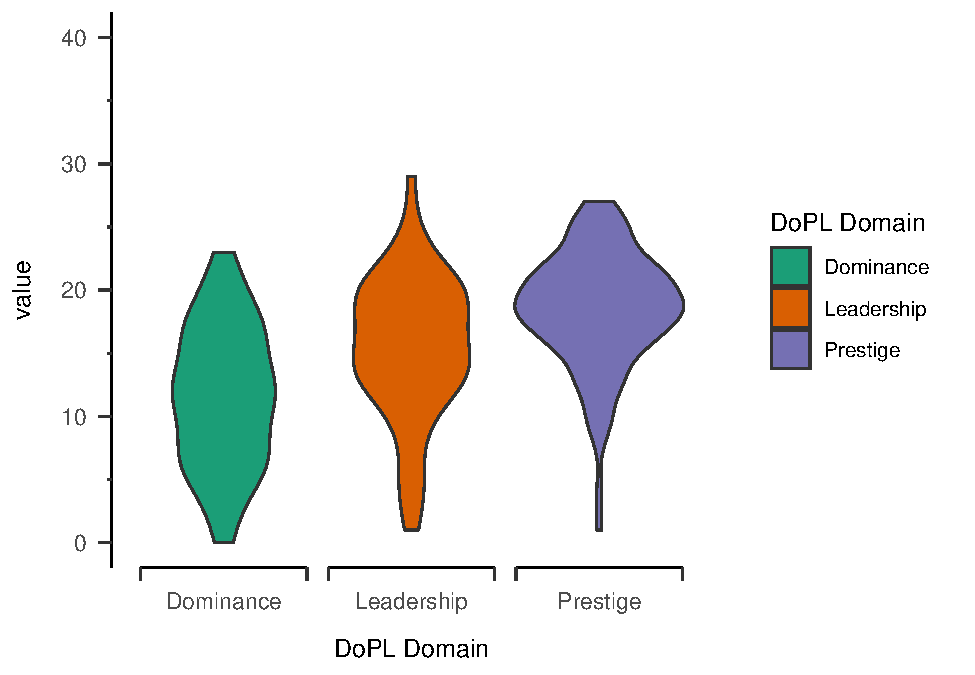
\includegraphics{Dissertation_files/figure-latex/Dominance, Prestige, and Leadership-1.pdf}
\caption{(\#fig:Dominance, Prestige, and Leadership)DoPL Domains distribution}
\end{figure}

\begin{figure}
\centering
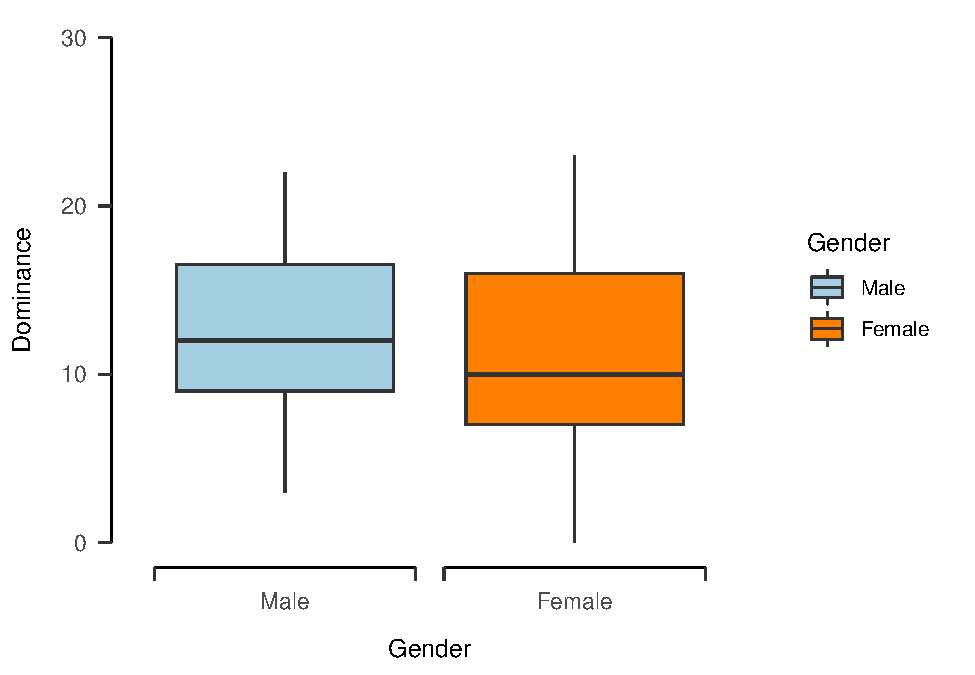
\includegraphics{Dissertation_files/figure-latex/Dominance-1.pdf}
\caption{\label{fig:Dominance}DoPL Domains distribution}
\end{figure}

\begin{figure}
\centering
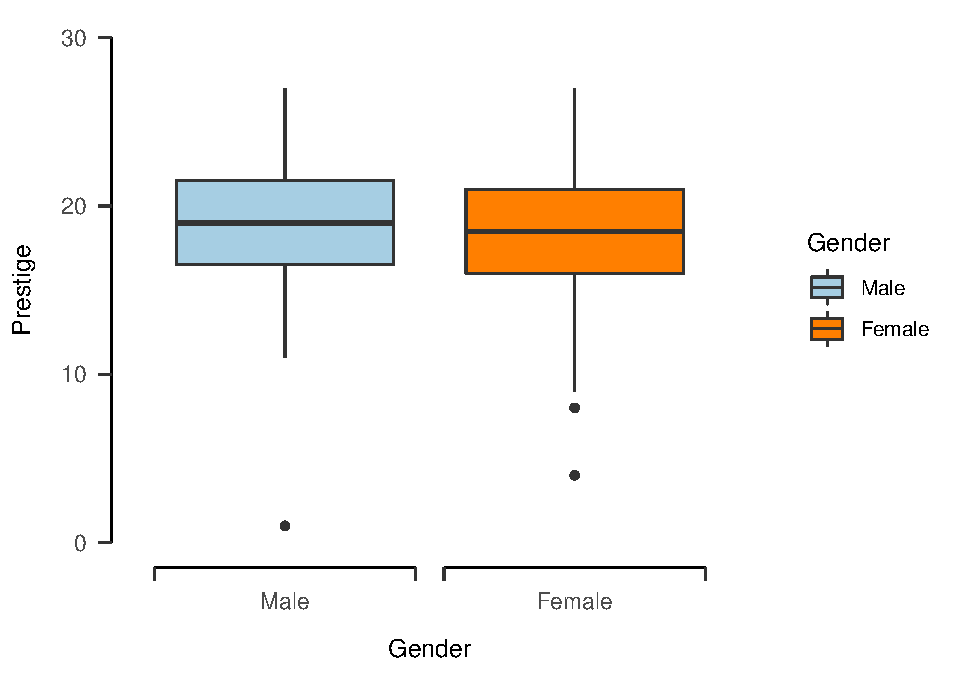
\includegraphics{Dissertation_files/figure-latex/Prestige-1.pdf}
\caption{\label{fig:Prestige}Prestige distribution}
\end{figure}

\begin{figure}
\centering
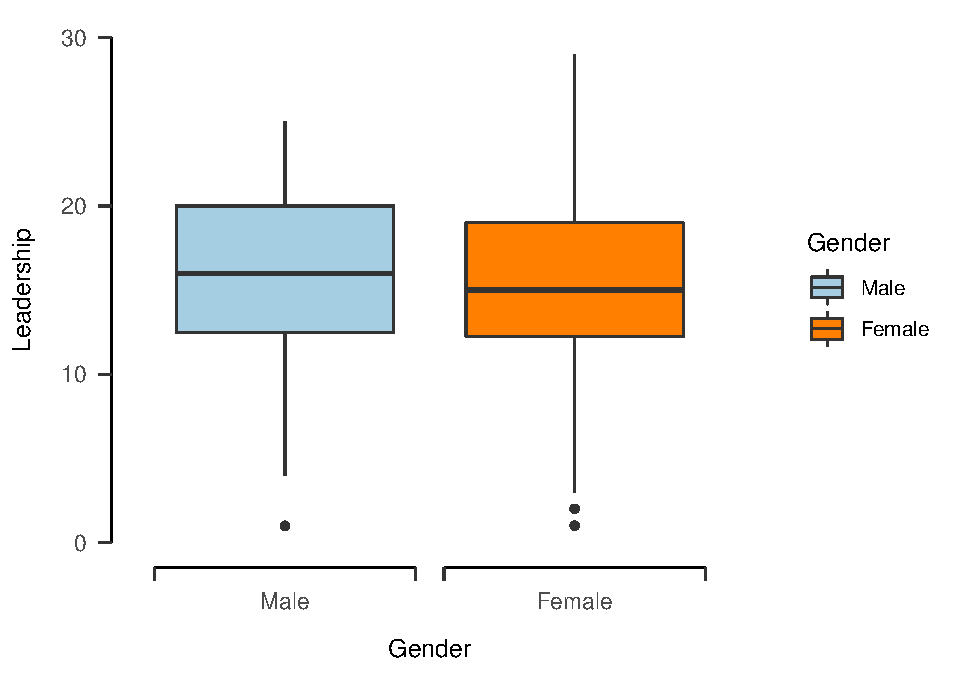
\includegraphics{Dissertation_files/figure-latex/Leadership-1.pdf}
\caption{\label{fig:Leadership}DoPL Domains distribution}
\end{figure}

\begin{table}[tbp]

\begin{center}
\begin{threeparttable}

\caption{\label{tab:fixed effects experiment 1}}

\begin{tabular}{lllll}
\toprule
 & \multicolumn{1}{c}{Estimate} & \multicolumn{1}{c}{Est.Error} & \multicolumn{1}{c}{Q2.5} & \multicolumn{1}{c}{Q97.5}\\
\midrule
Intercept & 3.62 & 1.13 & 1.41 & 5.86\\
dominanceSum & 3.00 & 0.99 & 1.08 & 4.93\\
prestigeSum & 0.09 & 0.99 & -1.84 & 2.02\\
leadershipSum & -1.91 & 0.98 & -3.85 & 0.02\\
Gender1 & -3.02 & 0.99 & -4.95 & -1.08\\
Age & -2.86 & 0.99 & -4.78 & -0.93\\
\bottomrule
\end{tabular}

\end{threeparttable}
\end{center}

\end{table}

\begin{table}[tbp]

\begin{center}
\begin{threeparttable}

\caption{\label{tab:HDI model 3}}

\begin{tabular}{llll}
\toprule
Parameter & \multicolumn{1}{c}{CI} & \multicolumn{1}{c}{CI\_low} & \multicolumn{1}{c}{CI\_high}\\
\midrule
b\_ethicalPreference\_Intercept & 0.95 & 2.85 & 4.42\\
b\_ethicalPreference\_dominanceSum & 0.95 & 0.61 & 1.71\\
b\_financialPreference\_Intercept & 0.95 & 7.50 & 9.67\\
b\_financialPreference\_dominanceSum & 0.95 & 0.14 & 1.59\\
b\_socialPreference\_Intercept & 0.95 & 8.34 & 11.67\\
b\_socialPreference\_dominanceSum & 0.95 & 0.60 & 2.87\\
b\_healthAndSafetyPreference\_Intercept & 0.95 & 4.65 & 6.59\\
b\_healthAndSafetyPreference\_dominanceSum & 0.95 & 0.41 & 1.77\\
b\_recreationalPreference\_Intercept & 0.95 & 0.95 & 2.48\\
b\_recreationalPreference\_dominanceSum & 0.95 & 0.66 & 1.74\\
b\_recreationalPreference\_Gender1 & 0.95 & -1.83 & -0.47\\
b\_recreationalPreference\_Age & 0.95 & 0.06 & 0.87\\
\bottomrule
\end{tabular}

\end{threeparttable}
\end{center}

\end{table}

\hypertarget{experiment-2-figures}{%
\section{Experiment 2: Figures}\label{experiment-2-figures}}

\begin{figure}
\centering
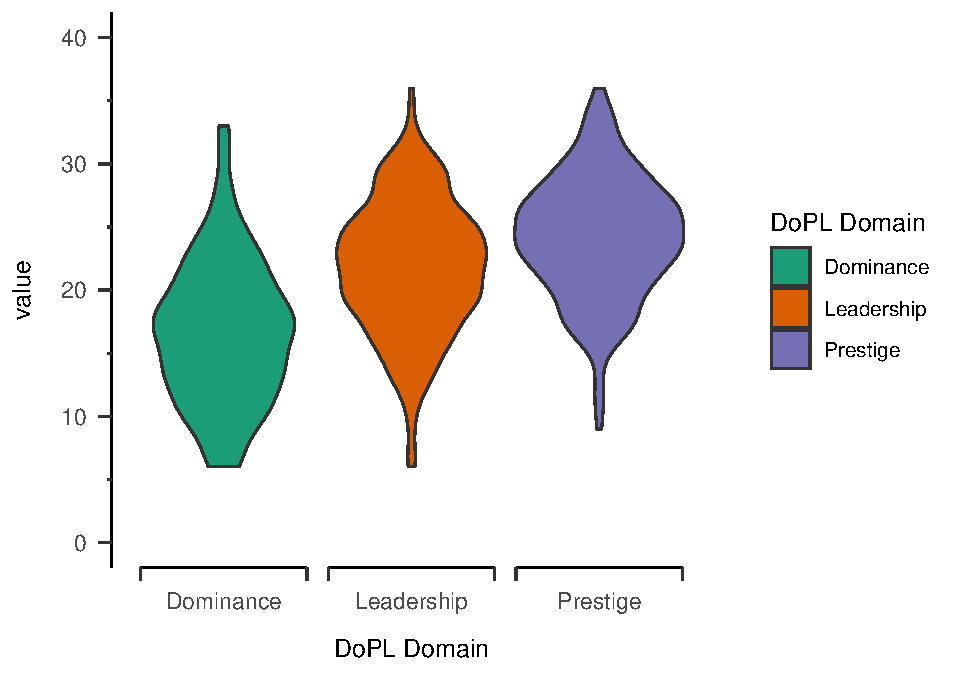
\includegraphics{Dissertation_files/figure-latex/DoPL Domains Experiment 2-1.pdf}
\caption{(\#fig:DoPL Domains Experiment 2)DoPL Domains Experiment 2}
\end{figure}

\hypertarget{chapter-3}{%
\section{Chapter 3:}\label{chapter-3}}

\hypertarget{experiment-1}{%
\subsection{Experiment 1:}\label{experiment-1}}

\hypertarget{experiment-1-review}{%
\subsection{Experiment 1 Review}\label{experiment-1-review}}

In an extension of the previous research, we sought other areas of possible interest in what could be affecting individuals' likelihood to engage in either immoral or risky behaviors. So far we have shown a connection with power motives such as Dominance, Prestige, and leadership (DoPL); along with investigating the connection between DoPL and the domain-specific risk-taking scale. An intriguing area that has not been extensively researched is narcissism. Personality research is often the viewpoint at which narcissism is investigated such as using the five-factor model concept where the primary traits are extraversion and agreeableness (Hyatt et al., 2018).

\hypertarget{narcissism}{%
\subsection{Narcissism}\label{narcissism}}

Narcissism is a personality trait that originally was seen as a method or mechanism to shield the individual from feelings of low self-worth (Yakeley, 2018). The understanding of what narcissism soon shifted with a focus on empirical understandings of the individual. Researchers such as Jeffrey Young, who expanded on the work of Aaron Beck, theorized that the core beliefs of an individual along with negative self-schemas influence the individual to seek out or act in ways in line with a narcissitic personality (J. E. Young et al., 2006). Conceptualizations of narcissism would soon entail it to be an understanding of grandiose sense of self, fantastical beliefs of success and general superiority, along with a general lack of empathy (American Psychiatric Association, 2013; Okada, 2010; Yakeley, 2018)./
The earliest understandings of narcissism were through Sigmund Freud. However, the term was first coined by Havelock Ellis who used the eponymous Narcissus myth in the explanation of narcissism. Freud would then publish the text \emph{On Narcissism} to further our understanding of narcissism. Future understandings of narcissism would develop from a social cognitive framework of the indvidual in relation to their environment. Such as Kernberg's assestment that narcissism stems from an aggressive and conflict filled childhood affecting the childs development and later aggression and envy towards others (Russell, 1985).

\begin{itemize}
\item
  note on the early understandings of how narcissism was interpreted as being, i.e., a defense mechanism Yakeley (2018)
\item
  continued lack of consensus on what consitutes narcissism Ackerman et al. (2017)

  \begin{itemize}
  \tightlist
  \item
    Also the discussion of social dominance in regard to narcissistic personality disorder Ackerman et al. (2017)
  \end{itemize}
\end{itemize}

\hypertarget{the-present-experiments}{%
\subsection{The present Experiments}\label{the-present-experiments}}

Pathological narcissism at it's core looks strikingly similar to self-esteem and in turn a grandiose sense of self. Investigations at risky situations have looked at sexual self-esteem, exploratory experiment one. The present experiment seeks to expand to investigate the relationship between pathological narcissism and see which is a stronger predictor of risky sexual situations and riskiness in general.

\hypertarget{methods-2}{%
\subsection{Methods}\label{methods-2}}

Participants were a convenience sample of 111 individuals from Prolific Academic's crowdsourcing platform (www.prolific.io). Prolific Academic is an online crowdsourcing service that provides participants access to studies hosted on third-party websites. Participants were required to be 18 years of age or older and be able to read and understand English. Participants received £4.00, which is above the current minimum wage pro-rata in the United Kingdom, as compensation for completing the survey. The Psychology Research Ethics Committee at the University of Edinburgh approved all study procedures {[}ref: 174-2122/5{]}. The present study was pre-registered along with a copy of anonymized data along with a copy of the R code and supplemental materials are available at (\url{https://osf.io/s4j7y}).

\hypertarget{materials-3}{%
\subsection{Materials}\label{materials-3}}

\hypertarget{demographic-questionnaire-3}{%
\subsubsection{\texorpdfstring{\emph{Demographic Questionnaire}}{Demographic Questionnaire}}\label{demographic-questionnaire-3}}

In a demographic questionnaire administered prior to the main survey, participants were invited to respond to a series of questions about their self-identified demographic characteristics such as age, gender, ethnicity, and ethnic origin.

\hypertarget{sexual-risk-taking-behavior-scale}{%
\subsubsection{\texorpdfstring{\emph{Sexual Risk-taking Behavior Scale}}{Sexual Risk-taking Behavior Scale}}\label{sexual-risk-taking-behavior-scale}}

The 54-item Sexual Risk-taking Behavior Scale (SRTB; Spiegel and Pollak (2019)), is a scale measuring individuals on their risk-taking by requesting they respond to a series of statements and their agreement on three different domains (i.e., Risk perception, likelihood, and benefit perception). They are then given a series of statements of sexual activities and the frequency that they have engaged in those behaviors. Example items for the first three domains are ``Sexual activity with multiple participants'' and ``Sex under influence of substances (drugs/alcohol).'' For frequency, participants are asked to rate each sexual behavior on a scale of never {[}1{]} to at least once a day {[}8{]}.

\hypertarget{sociosexual-orientation-inventory}{%
\subsubsection{\texorpdfstring{\emph{Sociosexual Orientation Inventory}}{Sociosexual Orientation Inventory}}\label{sociosexual-orientation-inventory}}

The Sociosexual Orientation Inventory (SOI-R; Penke and Asendorpf (2008)) is a 9 item scale asking participants a series of questions of how many times participants have engaged in the questioned sexual behaviors. Example items are ``With how many different partners have you had sex with in the past 12 months?'' and ``With how many different partners have you had sexual intercourse on one and only one occasion?'' rated on a scale from 0 to 20 or more.

\hypertarget{dominance-prestige-and-leadership}{%
\subsubsection{\texorpdfstring{\emph{Dominance, Prestige, and Leadership}}{Dominance, Prestige, and Leadership}}\label{dominance-prestige-and-leadership}}

The 18-item Dominance, Prestige, and Leadership scale (DoPL; Süssenbach and Bohner (2011)), measures dominance, prestige, and leadership orientation. Each question corresponds to one of the three domains. Each domain is scored across 6 unique items related to those domains (e.g., ``I relish opportunities in which I can lead others'' for leadership) rated on a scale from 0 (Strongly disagree) to 5 (Strongly agree).

\hypertarget{pathological-narcissism}{%
\subsubsection{\texorpdfstring{\emph{Pathological Narcissism}}{Pathological Narcissism}}\label{pathological-narcissism}}

The brief Pathological Narcissism Inventory (B-PNI; Schoenleber et al. (2015)) is a 28 item inventory measuring individuals on 7 aspects of pathological narcissism facet scales. Example items are ``I feel important when others rely on me'' and ``Sacrificing for others makes me the better person'' rated on a scale from 1 (not at all like me) to 5 (Very much like me).

\hypertarget{procedure-5}{%
\subsection{Procedure}\label{procedure-5}}

In study 2, participants were recruited via a study landing page on Prolific's website or via a direct e-mail to eligible participants (Prolific Academic, 2018). The study landing page included a brief description of the study including any risks and benefits along with expected compensation for successful completion. Participants accepted participation in the experiment and were directed to the main survey (Pavlovia.org) where they were shown a brief message on study consent.

Once participants consented to participate in the experiment they answered a series of demographic questions. Once completed, participants completed the Dominance, Prestige, and Leadership Scale and the Domain Specific Risk-taking scale. The two scales were counterbalanced to account for order effects. After completion of the main survey, participants were shown a debriefing statement that briefly mentions the purpose of the experiment along with the contact information of the main researcher (AI). Participants were compensated with course credit on the University of Edinburgh's SONA system.

\hypertarget{data-analysis-5}{%
\subsection{Data analysis}\label{data-analysis-5}}

Demographic characteristics were analyzed using multiple regression for continuous variables (age) and Chi-square tests for categorical variables (gender, race, ethnicity, ethnic origin, and education). Means and standard deviations were calculated for the relevant scales (i.e., DoPL and SRTB). All analyses were done using (R Core Team, 2021) along with (Bürkner, 2017) package.

The use of bayesian statistics has a multitude of benefits to statistical analysis and research design. One important benefit is through the use of prior data in future analyses. Termed as priors, is the use of prior distributions for future analysis. This allows for the separation of how the data might have been collected or what the intention was. In essence, the data is the data without the interpretation of the scientist.

All relevant analyses were conducted in a Bayesian framework using the brms package (Bürkner, 2018) along with the cmdstanr packages notes (Gabry \& Cesnovar, 2021). In addition to the aforementioned packages, we used bayestestR, rstan, and papaja for further analysis and creation of this manuscript (Aust \& Barth, 2020; Makowski et al., 2019; Stan Development Team, 2020).

\hypertarget{results-2}{%
\subsection{Results}\label{results-2}}

\hypertarget{preregistered-analyses-3}{%
\subsubsection{Preregistered Analyses}\label{preregistered-analyses-3}}

\hypertarget{demographic-and-dopl-2}{%
\subsubsection{\texorpdfstring{\emph{Demographic and DoPL}}{Demographic and DoPL}}\label{demographic-and-dopl-2}}

\hypertarget{domain-specific-risk-taking-3}{%
\subsection{Domain-Specific Risk-Taking}\label{domain-specific-risk-taking-3}}

\hypertarget{interactions-3}{%
\subsection{Interactions}\label{interactions-3}}

\hypertarget{discussion-2}{%
\subsection{Discussion}\label{discussion-2}}

\newpage

\hypertarget{references}{%
\section{References}\label{references}}

\begingroup
\setlength{\parindent}{-0.5in}
\setlength{\leftskip}{0.5in}

\hypertarget{refs}{}
\begin{CSLReferences}{1}{0}
\leavevmode\vadjust pre{\hypertarget{ref-abelson1981}{}}%
Abelson, R. P. (1981). Psychological status of the script concept. \emph{American Psychologist}, \emph{36}(7), 715--729. \url{https://doi.org/10.1037/0003-066X.36.7.715}

\leavevmode\vadjust pre{\hypertarget{ref-ackerman2017}{}}%
Ackerman, R. A., Hands, A. J., Donnellan, M. B., Hopwood, C. J., \& Witt, E. A. (2017). Experts' views regarding the conceptualization of narcissism. \emph{Journal of Personality Disorders}, \emph{31}(3), 346--361. \url{https://doi.org/gbhhv3}

\leavevmode\vadjust pre{\hypertarget{ref-americanpsychiatricassociation2013}{}}%
American Psychiatric Association. (2013). \emph{Diagnostic and Statistical Manual of Mental Disorders} (Fifth Edition). American Psychiatric Association. \url{https://doi.org/10.1176/appi.books.9780890425596}

\leavevmode\vadjust pre{\hypertarget{ref-andersen1994}{}}%
Andersen, B. L., Cyranowski, J. M., \& Espindle, D. (1994). \emph{Women's sexual self-schema.} \url{https://doi.org/10.1037/0022-3514.67.6.1079}

\leavevmode\vadjust pre{\hypertarget{ref-andersen1999}{}}%
Andersen, B. L., Cyranowski, J. M., \& Espindle, D. (1999). Men's sexual self-schema. \emph{Journal of Personality and Social Psychology}, \emph{76}(4), 645--661. \url{https://doi.org/10.1037/0022-3514.76.4.645}

\leavevmode\vadjust pre{\hypertarget{ref-anderson2002}{}}%
Anderson, C. A., \& Bushman, B. J. (2002). Human aggression. \emph{Annual Review of Psychology}, \emph{53}(1), 27--51. \url{https://doi.org/10.1146/annurev.psych.53.100901.135231}

\leavevmode\vadjust pre{\hypertarget{ref-anderson2012}{}}%
Anderson, C., John, O. P., \& Keltner, D. (2012). The personal sense of power. \emph{Journal of Personality}, \emph{80}(2), 313--344. \url{https://doi.org/10.1111/j.1467-6494.2011.00734.x}

\leavevmode\vadjust pre{\hypertarget{ref-aristotle1984}{}}%
Aristotle. (1984). \emph{Complete works of aristotle, volume 2: the revised oxford translation}. Princeton University Press.

\leavevmode\vadjust pre{\hypertarget{ref-aust2020}{}}%
Aust, F., \& Barth, M. (2020). \emph{papaja: Prepare reproducible APA journal articles with R Markdown} {[}R{]}. \url{https://github.com/crsh/papaja}

\leavevmode\vadjust pre{\hypertarget{ref-bareket2020}{}}%
Bareket, O., \& Shnabel, N. (2020). Domination and objectification: men's motivation for dominance over women affects their tendency to sexually objectify women. \emph{Psychology of Women Quarterly}, \emph{44}(1), 28--49. \url{https://doi.org/10.1177/0361684319871913}

\leavevmode\vadjust pre{\hypertarget{ref-barnett2013}{}}%
Barnett, G. D., \& Mann, R. E. (2013). Cognition, empathy, and sexual offending. \emph{Trauma, Violence, \& Abuse}, \emph{14}(1), 22--33. \url{https://doi.org/10.1177/1524838012467857}

\leavevmode\vadjust pre{\hypertarget{ref-bastian2010}{}}%
Bastian, B., \& Haslam, N. (2010). Excluded from humanity: the dehumanizing effects of social ostracism. \emph{Journal of Experimental Social Psychology}, \emph{46}(1), 107--113. \url{https://doi.org/10.1016/j.jesp.2009.06.022}

\leavevmode\vadjust pre{\hypertarget{ref-bastian2013}{}}%
Bastian, B., Jetten, J., Chen, H., Radke, H. R. M., Harding, J. F., \& Fasoli, F. (2013). Losing our humanity: the self-dehumanizing consequences of social ostracism. \emph{Personality \& Social Psychology Bulletin}, \emph{39}(2), 156--169. \url{https://doi.org/10.1177/0146167212471205}

\leavevmode\vadjust pre{\hypertarget{ref-bastian2012}{}}%
Bastian, B., Jetten, J., \& Radke, H. R. M. (2012). Cyber-dehumanization: violent video game play diminishes our humanity. \emph{Journal of Experimental Social Psychology}, \emph{48}(2), 486--491. \url{https://doi.org/10.1016/j.jesp.2011.10.009}

\leavevmode\vadjust pre{\hypertarget{ref-bernstein2020}{}}%
Bernstein, R. (2020, February 22). The paradox of rodrigo duterte. \emph{The Atlantic}. \url{https://www.theatlantic.com/international/archive/2020/02/philippines-rodrigo-duterte-china/606754/}

\leavevmode\vadjust pre{\hypertarget{ref-bierstedt1950}{}}%
Bierstedt, R. (1950). An analysis of social power. \emph{American Sociological Review}, \emph{15}(6), 730--738. JSTOR. \url{https://doi.org/10.2307/2086605}

\leavevmode\vadjust pre{\hypertarget{ref-breakwell2007}{}}%
Breakwell, G. M. (2007, November). \emph{The psychology of risk}. \url{https://doi.org/10.1017/CBO9780511819315}

\leavevmode\vadjust pre{\hypertarget{ref-bugental2002}{}}%
Bugental, D. B., \& Shennum, W. (2002). Gender, power, and violence in the family. \emph{Child Maltreatment}, \emph{7}(1), 55--63. \url{https://doi.org/10.1177/1077559502007001005}

\leavevmode\vadjust pre{\hypertarget{ref-burkner2017}{}}%
Bürkner, P.-C. (2017). brms: an R package for bayesian multilevel models using stan. \emph{Journal of Statistical Software}, \emph{80}(1), 1--28. \url{https://doi.org/10.18637/jss.v080.i01}

\leavevmode\vadjust pre{\hypertarget{ref-burkner2018}{}}%
Bürkner, P.-C. (2018). Advanced bayesian multilevel modeling with the R package brms. \emph{The R Journal}, \emph{10}(1), 395--411. \url{https://doi.org/10.32614/RJ-2018-017}

\leavevmode\vadjust pre{\hypertarget{ref-byom2013}{}}%
Byom, L. J., \& Mutlu, B. (2013). Theory of mind: mechanisms, methods, and new directions. \emph{Frontiers in Human Neuroscience}, \emph{7}. \url{https://doi.org/10.3389/fnhum.2013.00413}

\leavevmode\vadjust pre{\hypertarget{ref-carmonagutierrez2016}{}}%
Carmona-Gutierrez, D., Kainz, K., \& Madeo, F. (2016). Sexually transmitted infections: old foes on the rise. \emph{Microbial Cell}, \emph{3}(9), 361--362. \url{https://doi.org/10.15698/mic2016.09.522}

\leavevmode\vadjust pre{\hypertarget{ref-castrovazquez2000}{}}%
Castro-Vázquez, G. (2000). Masculinity and condom use among mexican teenagers: the escuela nacional preparatoria no. 1's case. \emph{Gender and Education}, \emph{12}(4), 479--492. \url{https://doi.org/10.1080/09540250020004117}

\leavevmode\vadjust pre{\hypertarget{ref-chen2021}{}}%
Chen, Z., \& John, R. S. (2021). Decision heuristics and descriptive choice models for sequential high-stakes risky choices in the deal or no deal game. \emph{Decision}, \emph{8}(3), 155--179. \url{https://doi.org/10.1037/dec0000153}

\leavevmode\vadjust pre{\hypertarget{ref-chiappori2019}{}}%
Chiappori, P.-A., \& Molina, J. A. (2019). \emph{1 the intra-spousal balance of power within the family : cross-cultural evidence}.

\leavevmode\vadjust pre{\hypertarget{ref-clifford2015}{}}%
Clifford, S., Iyengar, V., Cabeza, R., \& Sinnott-Armstrong, W. (2015). Moral foundations vignettes: a standardized stimulus database of scenarios based on moral foundations theory. \emph{Behavior Research Methods}, \emph{47}(4), 1178--1198. \url{https://doi.org/10.3758/s13428-014-0551-2}

\leavevmode\vadjust pre{\hypertarget{ref-costalourenco2017}{}}%
Costa-Lourenço, A. P. R. da, Barros dos Santos, K. T., Moreira, B. M., Fracalanzza, S. E. L., \& Bonelli, R. R. (2017). Antimicrobial resistance in neisseria gonorrhoeae: history, molecular mechanisms and epidemiological aspects of an emerging global threat. \emph{Brazilian Journal of Microbiology}, \emph{48}(4), 617--628. \url{https://doi.org/10.1016/j.bjm.2017.06.001}

\leavevmode\vadjust pre{\hypertarget{ref-cowan1999}{}}%
Cowan, N. (1999). An embedded-processes model of working memory. In A. Miyake \& P. Shah (Eds.), \emph{Models of Working Memory} (1st ed., pp. 62--101). Cambridge University Press. \url{https://doi.org/10.1017/CBO9781139174909.006}

\leavevmode\vadjust pre{\hypertarget{ref-crandall2017}{}}%
Crandall, A., Magnusson, B., Novilla, M., Novilla, L. K. B., \& Dyer, W. (2017). Family financial stress and adolescent sexual risk-taking: the role of self-regulation. \emph{Journal of Youth and Adolescence}, \emph{46}(1), 45--62. \url{https://doi.org/10.1007/s10964-016-0543-x}

\leavevmode\vadjust pre{\hypertarget{ref-cunningham2009}{}}%
Cunningham, S. D., Kerrigan, D. L., Jennings, J. M., \& Ellen, J. M. (2009). Relationships between perceived std-related stigma, std-related shame and std screening among a household sample of adolescents. \emph{Perspectives on Sexual and Reproductive Health}, \emph{41}(4), 225--230. \url{https://doi.org/10.1363/4122509}

\leavevmode\vadjust pre{\hypertarget{ref-cyranowski1999}{}}%
CYRANOWSKI, J. M., AARESTAD, S. L., \& ANDERSEN, B. L. (1999). The role of sexual self-schema in a diathesis--stress model of sexual dysfunction. \emph{Applied \& Preventive Psychology : Journal of the American Association of Applied and Preventive Psychology}, \emph{8}(3), 217--228. \url{https://doi.org/10.1016/S0962-1849(05)80078-2}

\leavevmode\vadjust pre{\hypertarget{ref-desanjose2008}{}}%
de Sanjose, S., Cortés, X., Méndez, C., Puig-Tintore, L., Torné, A., Roura, E., Bosch, F. X., \& Castellsague, X. (2008). Age at sexual initiation and number of sexual partners in the female spanish population: results from the AFRODITA survey. \emph{European Journal of Obstetrics \& Gynecology and Reproductive Biology}, \emph{140}(2), 234--240. \url{https://doi.org/10.1016/j.ejogrb.2008.04.005}

\leavevmode\vadjust pre{\hypertarget{ref-desiderato1995}{}}%
Desiderato, L. L., \& Crawford, H. J. (1995). Risky sexual behavior in college students: relationships between number of sexual partners, disclosure of previous risky behavior, and alcohol use. \emph{Journal of Youth and Adolescence}, \emph{24}(1), 55--68. \url{https://doi.org/10.1007/BF01537560}

\leavevmode\vadjust pre{\hypertarget{ref-dickson1998}{}}%
Dickson, N., Paul, C., Herbison, P., \& Silva, P. (1998). First sexual intercourse: age, coercion, and later regrets reported by a birth cohort. \emph{BMJ}, \emph{316}(7124), 29--33. \url{https://doi.org/10.1136/bmj.316.7124.29}

\leavevmode\vadjust pre{\hypertarget{ref-dimaggio1997}{}}%
DiMaggio, P. (1997). Culture and cognition. \emph{Annual Review of Sociology}, \emph{23}(1), 263--287. \url{https://doi.org/10.1146/annurev.soc.23.1.263}

\leavevmode\vadjust pre{\hypertarget{ref-elder2012}{}}%
Elder, W. B., Brooks, G. R., \& Morrow, S. L. (2012). Sexual self-schemas of heterosexual men. \emph{Psychology of Men \& Masculinity}, \emph{13}(2), 166--179. \url{https://doi.org/10.1037/a0024835}

\leavevmode\vadjust pre{\hypertarget{ref-elder2015a}{}}%
Elder, W. B., Morrow, S. L., \& Brooks, G. R. (2015). Sexual self-schemas of gay men: a qualitative investigation. \emph{The Counseling Psychologist}, \emph{43}(7), 942--969. \url{https://doi.org/10.1177/0011000015606222}

\leavevmode\vadjust pre{\hypertarget{ref-ellemers2019}{}}%
Ellemers, N., van der Toorn, J., Paunov, Y., \& van Leeuwen, T. (2019). The psychology of morality: A review and analysis of empirical studies published from 1940 through 2017. \emph{Personality and Social Psychology Review}, \emph{23}(4), 332--366. \url{https://doi.org/10.1177/1088868318811759}

\leavevmode\vadjust pre{\hypertarget{ref-ellis2004}{}}%
Ellis, V., \& High, S. (2004). Something more to tell you: gay, lesbian or bisexual young people's experiences of secondary schooling. \emph{British Educational Research Journal}, \emph{30}(2), 213--225. \url{https://doi.org/10.1080/0141192042000195281}

\leavevmode\vadjust pre{\hypertarget{ref-eskine2011}{}}%
Eskine, K. J., Kacinik, N. A., \& Prinz, J. J. (2011). A bad taste in the mouth: gustatory disgust influences moral judgment. \emph{Psychological Science}, \emph{22}(3), 295--299. \url{https://doi.org/10.1177/0956797611398497}

\leavevmode\vadjust pre{\hypertarget{ref-festinger1957}{}}%
Festinger, L. (1957). \emph{A theory of cognitive dissonance} (pp. xi, 291). Stanford University Press.

\leavevmode\vadjust pre{\hypertarget{ref-finucane2000}{}}%
Finucane, M. L., Alhakami, A., Slovic, P., \& Johnson, S. M. (2000). The affect heuristic in judgments of risks and benefits. \emph{Journal of Behavioral Decision Making}, \emph{13}(1), 1--17. \url{https://doi.org/10.1002/(SICI)1099-0771(200001/03)13:1\%3C1::AID-BDM333\%3E3.0.CO;2-S}

\leavevmode\vadjust pre{\hypertarget{ref-gabry2021}{}}%
Gabry, J., \& Cesnovar, R. (2021). \emph{cmdstanr: R interface to {``CmdStan''}} {[}R{]}. \href{https://mc-stan.org/cmdstanr,\%20https://discourse.mc-stan.org}{https://mc-stan.org/cmdstanr, https://discourse.mc-stan.org}

\leavevmode\vadjust pre{\hypertarget{ref-gannon2009}{}}%
Gannon, T. A. (2009). Social cognition in violent and sexual offending: an overview. \emph{Psychology, Crime \& Law}, \emph{15}(2-3), 97--118. \url{https://doi.org/10.1080/10683160802190822}

\leavevmode\vadjust pre{\hypertarget{ref-gesink2016}{}}%
Gesink, D., Whiskeyjack, L., Suntjens, T., Mihic, A., \& McGilvery, P. (2016). Abuse of power in relationships and sexual health. \emph{Child Abuse \& Neglect}, \emph{58}, 12--23. \url{https://doi.org/10.1016/j.chiabu.2016.06.005}

\leavevmode\vadjust pre{\hypertarget{ref-2018}{}}%
Glamorizing dictators. (2018, February 22). \emph{Towson University Journal of International Affairs}. \url{https://wp.towson.edu/iajournal/2018/02/21/glamorizing-dictators/}

\leavevmode\vadjust pre{\hypertarget{ref-glenn2009}{}}%
Glenn, A. L., Raine, A., \& Schug, R. A. (2009). The neural correlates of moral decision-making in psychopathy. \emph{Molecular Psychiatry}, \emph{14}(1), 5--6. \url{https://doi.org/10.1038/mp.2008.104}

\leavevmode\vadjust pre{\hypertarget{ref-graham2011}{}}%
Graham, J., Nosek, B. A., Haidt, J., Iyer, R., Koleva, S., \& Ditto, P. H. (2011). Mapping the moral domain. \emph{Journal of Personality and Social Psychology}, \emph{101}(2), 366--385. \url{https://doi.org/10.1037/a0021847}

\leavevmode\vadjust pre{\hypertarget{ref-greenberg1990}{}}%
Greenberg, J., Pyszczynski, T., Solomon, S., Rosenblatt, A., \& et al. (1990). Evidence for terror management theory II: the effects of mortality salience on reactions to those who threaten or bolster the cultural worldview. \emph{Journal of Personality and Social Psychology}, \emph{58}(2), 308--318. \url{https://doi.org/10.1037/0022-3514.58.2.308}

\leavevmode\vadjust pre{\hypertarget{ref-greene2001}{}}%
Greene, J. D. (2001). An fMRI investigation of emotional engagement in moral judgment. \emph{Science}, \emph{293}(5537), 2105--2108. \url{https://doi.org/10.1126/science.1062872}

\leavevmode\vadjust pre{\hypertarget{ref-gwinn2013}{}}%
Gwinn, J. D., Judd, C. M., \& Park, B. (2013). Less power = less human? Effects of power differentials on dehumanization. \emph{Journal of Experimental Social Psychology}, \emph{49}(3), 464--470. \url{https://doi.org/10.1016/j.jesp.2013.01.005}

\leavevmode\vadjust pre{\hypertarget{ref-haidt2001}{}}%
Haidt, J. (2001). The emotional dog and its rational tail: A social intuitionist approach to moral judgment. \emph{Psychological Review}, \emph{108}(4), 814--834. \url{https://doi.org/10.1037/0033-295X.108.4.814}

\leavevmode\vadjust pre{\hypertarget{ref-haslam2014}{}}%
Haslam, N., \& Loughnan, S. (2014). Dehumanization and infrahumanization. \emph{Annual Review of Psychology}, \emph{65}(1), 399--423. \url{https://doi.org/10.1146/annurev-psych-010213-115045}

\leavevmode\vadjust pre{\hypertarget{ref-horberg2009}{}}%
Horberg, E. J., Oveis, C., Keltner, D., \& Cohen, A. B. (2009). Disgust and the moralization of purity. \emph{Journal of Personality and Social Psychology}, \emph{97}(6), 963--976. \url{https://doi.org/10.1037/a0017423}

\leavevmode\vadjust pre{\hypertarget{ref-hyatt2018}{}}%
Hyatt, C. S., Sleep, C. E., Lamkin, J., Maples-Keller, J. L., Sedikides, C., Campbell, W. K., \& Miller, J. D. (2018). Narcissism and self-esteem: A nomological network analysis. \emph{PLOS ONE}, \emph{13}(8), e0201088. \url{https://doi.org/gdzd3c}

\leavevmode\vadjust pre{\hypertarget{ref-ison2011}{}}%
Ison, C. A., \& Alexander, S. (2011). Antimicrobial resistance in neisseria gonorrhoeae in the UK: surveillance and management. \emph{Expert Review of Anti-Infective Therapy}, \emph{9}(10), 867--876. \url{https://doi.org/10.1586/eri.11.103}

\leavevmode\vadjust pre{\hypertarget{ref-johnson2012}{}}%
Johnson, M. W., \& Bruner, N. R. (2012). The sexual discounting task: HIV risk behavior and the discounting of delayed sexual rewards in cocaine dependence. \emph{Drug and Alcohol Dependence}, \emph{123}(1-3), 15--21. \url{https://doi.org/10.1016/j.drugalcdep.2011.09.032}

\leavevmode\vadjust pre{\hypertarget{ref-johnson2015a}{}}%
Johnson, P. S., Herrmann, E. S., \& Johnson, M. W. (2015). Opportunity costs of reward delays and the discounting of hypothetical money and cigarettes: OPPORTUNITY COSTS AND DISCOUNTING. \emph{Journal of the Experimental Analysis of Behavior}, \emph{103}(1), 87--107. \url{https://doi.org/10.1002/jeab.110}

\leavevmode\vadjust pre{\hypertarget{ref-kahneman1972}{}}%
Kahneman, D., \& Tversky, A. (1972). Subjective probability: A judgment of representativeness. \emph{Cognitive Psychology}, \emph{3}(3), 430--454. \url{https://doi.org/cmf8m8}

\leavevmode\vadjust pre{\hypertarget{ref-kilimnik2018}{}}%
Kilimnik, C. D., Boyd, R. L., Stanton, A. M., \& Meston, C. M. (2018). Identification of nonconsensual sexual experiences and the sexual self-schemas of women: implications for sexual functioning. \emph{Archives of Sexual Behavior}, \emph{47}(6), 1633--1647. \url{https://doi.org/10.1007/s10508-018-1229-0}

\leavevmode\vadjust pre{\hypertarget{ref-kim2020}{}}%
Kim, H. M., \& Miller, L. C. (2020). Are insecure attachment styles related to risky sexual behavior? A meta-analysis. \emph{Health Psychology: Official Journal of the Division of Health Psychology, American Psychological Association}, \emph{39}(1), 46--57. \url{https://doi.org/10.1037/hea0000821}

\leavevmode\vadjust pre{\hypertarget{ref-king2009}{}}%
King, A. J., Johnson, D. D. P., \& Van Vugt, M. (2009). The origins and evolution of leadership. \emph{Current Biology}, \emph{19}(19), R911--R916. \url{https://doi.org/10.1016/j.cub.2009.07.027}

\leavevmode\vadjust pre{\hypertarget{ref-kirby2007}{}}%
Kirby, D. B., Laris, B. A., \& Rolleri, L. A. (2007). Sex and HIV education programs: their impact on sexual behaviors of young people throughout the world. \emph{Journal of Adolescent Health}, \emph{40}(3), 206--217. \url{https://doi.org/10.1016/j.jadohealth.2006.11.143}

\leavevmode\vadjust pre{\hypertarget{ref-kirby2021}{}}%
Kirby, M. (2021). North korea on the brink of the biden administration: human rights, peace, and security. \emph{Indiana International \& Comparative Law Review}, \emph{31}(2), 309--327. \url{http://journals.iupui.edu/index.php/iiclr/article/view/25607}

\leavevmode\vadjust pre{\hypertarget{ref-kouchaki2018}{}}%
Kouchaki, M., Dobson, K. S. H., Waytz, A., \& Kteily, N. S. (2018). The link between self-dehumanization and immoral behavior. \emph{Psychological Science}, \emph{29}(8), 1234--1246. \url{https://doi.org/10.1177/0956797618760784}

\leavevmode\vadjust pre{\hypertarget{ref-kuhberger2009}{}}%
Kühberger, A., \& Tanner, C. (2009). Risky choice framing: task versions and a comparison of prospect theory and fuzzy-trace theory. \emph{Journal of Behavioral Decision Making}, \emph{23}(3), 314--329. \url{https://doi.org/dtqksm}

\leavevmode\vadjust pre{\hypertarget{ref-laakasuo2017}{}}%
Laakasuo, M., Sundvall, J., \& Drosinou, M. (2017). Individual differences in moral disgust do not predict utilitarian judgments, sexual and pathogen disgust do. \emph{Scientific Reports}, \emph{7}(1), 45526. \url{https://doi.org/10.1038/srep45526}

\leavevmode\vadjust pre{\hypertarget{ref-lammers2011}{}}%
Lammers, J., \& Stapel, D. A. (2011). Power increases dehumanization. \emph{Group Processes \& Intergroup Relations}, \emph{14}(1), 113--126. \url{https://doi.org/10.1177/1368430210370042}

\leavevmode\vadjust pre{\hypertarget{ref-macphail2001}{}}%
MacPhail, C., \& Campbell, C. (2001). {``I think condoms are good but, aai, I hate those things''}: \emph{Social Science \& Medicine}, \emph{52}(11), 1613--1627. \url{https://doi.org/10.1016/S0277-9536(00)00272-0}

\leavevmode\vadjust pre{\hypertarget{ref-makowski2019}{}}%
Makowski, D., Ben-Shachar, M., \& Ludecke, D. (2019). bayestestR: Describing Effects and their Uncertainty, Existence and Significance within the Bayesian Framework. \emph{Journal of Open Source Software}, \emph{4}(40). \url{https://doi.org/10.21105/joss.01541}

\leavevmode\vadjust pre{\hypertarget{ref-malamuth1996}{}}%
Malamuth, N. M., Heavey, C. L., \& Linz, D. (1996). The confluence model of sexual aggression. \emph{Journal of Offender Rehabilitation}, \emph{23}(3-4), 13--37. \url{https://doi.org/10.1300/J076v23n03_03}

\leavevmode\vadjust pre{\hypertarget{ref-malamuth1995}{}}%
Malamuth, N. M., Linz, D., Heavey, C. L., Barnes, G., \& Acker, M. (1995). Using the confluence model of sexual aggression to predict men's conflict with women: A 10-year follow-up study. \emph{Journal of Personality and Social Psychology}, \emph{69}(2), 353--369. \url{https://doi.org/10.1037/0022-3514.69.2.353}

\leavevmode\vadjust pre{\hypertarget{ref-maner2016}{}}%
Maner, J. K., \& Case, C. R. (2016). Dominance and prestige. In \emph{Advances in Experimental Social Psychology} (Vol. 54, pp. 129--180). Elsevier. \url{https://doi.org/10.1016/bs.aesp.2016.02.001}

\leavevmode\vadjust pre{\hypertarget{ref-marcus2014}{}}%
Marcus, D. K., Zeigler-Hill, V., Mercer, S. H., \& Norris, A. L. (2014). The psychology of spite and the measurement of spitefulness. \emph{Psychological Assessment}, \emph{26}(2), 563--574. \url{https://doi.org/10.1037/a0036039}

\leavevmode\vadjust pre{\hypertarget{ref-marcus2000}{}}%
Marcus, G. (2000). Emotions in politics. \emph{Annual Review of Political Science - ANNU REV POLIT SCI}, \emph{3}, 221--250. \url{https://doi.org/10.1146/annurev.polisci.3.1.221}

\leavevmode\vadjust pre{\hypertarget{ref-marshall1993}{}}%
Marshall, W. L., Hudson, S. M., \& Hodkinson, S. (1993). The importance of attachment bonds in the development of juvenile sex offending. In \emph{The juvenile sex offender.} (pp. 164--181). Guilford Press.

\leavevmode\vadjust pre{\hypertarget{ref-mercer2013}{}}%
Mercer, C. H., Tanton, C., Prah, P., Erens, B., Sonnenberg, P., Clifton, S., Macdowall, W., Lewis, R., Field, N., Datta, J., Copas, A. J., Phelps, A., Wellings, K., \& Johnson, A. M. (2013). Changes in sexual attitudes and lifestyles in britain through the life course and over time: findings from the national surveys of sexual attitudes and lifestyles (natsal). \emph{The Lancet}, \emph{382}(9907), 1781--1794. \url{https://doi.org/10.1016/S0140-6736(13)62035-8}

\leavevmode\vadjust pre{\hypertarget{ref-moll2005}{}}%
Moll, J., Zahn, R., de Oliveira-Souza, R., Krueger, F., \& Grafman, J. (2005). The neural basis of human moral cognition. \emph{Nature Reviews Neuroscience}, \emph{6}(10), 799--809. \url{https://doi.org/10.1038/nrn1768}

\leavevmode\vadjust pre{\hypertarget{ref-nationaleparis1793}{}}%
Nationale (Paris), C. (1793). \emph{Collection générale des décrets rendus par la convention nationale}. chez Baudouin.

\leavevmode\vadjust pre{\hypertarget{ref-okada2010}{}}%
Okada, R. (2010). The relationship between vulnerable narcissism and aggression in japanese undergraduate students. \emph{Personality and Individual Differences}, \emph{49}(2), 113--118. \url{https://doi.org/c73zz7}

\leavevmode\vadjust pre{\hypertarget{ref-papanek1972}{}}%
Papanek, H. (1972). Pathology of power striving and its treatment. \emph{Journal of Individual Psychology; Chicago, Ill.}, \emph{28}(1), 25--32. \url{http://search.proquest.com/docview/1303447697/citation/C0139F0ECA044577PQ/1}

\leavevmode\vadjust pre{\hypertarget{ref-penke2008}{}}%
Penke, L., \& Asendorpf, J. B. (2008). Beyond global sociosexual orientations: A more differentiated look at sociosexuality and its effects on courtship and romantic relationships. \emph{Journal of Personality and Social Psychology}, \emph{95}(5), 1113--1135. \url{https://doi.org/10.1037/0022-3514.95.5.1113}

\leavevmode\vadjust pre{\hypertarget{ref-petersen2018}{}}%
Petersen, R. M., Dubuc, C., \& Higham, J. P. (2018). Facial displays of dominance in non-human primates. In C. Senior (Ed.), \emph{The Facial Displays of Leaders} (pp. 123--143). Springer International Publishing. \url{https://doi.org/10.1007/978-3-319-94535-4_6}

\leavevmode\vadjust pre{\hypertarget{ref-pewresearchcenter2019}{}}%
Pew Research Center. (2019). \emph{Views on race in america 2019}. Pew Research Center, Washinton, D.C. \url{https://www.pewresearch.org/social-trends/2019/04/09/race-in-america-2019/}

\leavevmode\vadjust pre{\hypertarget{ref-pincus2009}{}}%
Pincus, A. L., Ansell, E. B., Pimentel, C. A., Cain, N. M., Wright, A. G. C., \& Levy, K. N. (2009). Initial construction and validation of the Pathological Narcissism Inventory. \emph{Psychological Assessment}, \emph{21}(3), 365--379. \url{https://doi.org/10.1037/a0016530}

\leavevmode\vadjust pre{\hypertarget{ref-pleck1993}{}}%
Pleck, J., Sonenstein, F., \& Ku, L. (1993). Masculinity ideology: its impact on adolescent males' heterosexual relationships. \emph{Journal of Social Issues}, \emph{49}(3), 19. \url{https://doi.org/10.1111/j.1540-4560.1993.tb01166.x}

\leavevmode\vadjust pre{\hypertarget{ref-prolificacademic2018}{}}%
Prolific Academic. (2018). \emph{How do participants find out about my study?} \url{https://researcher-help.prolific.co/hc/en-gb/articles/360009221253-How-do-participants-find-out-about-my-study-}

\leavevmode\vadjust pre{\hypertarget{ref-pulerwitz2000}{}}%
Pulerwitz, J., Gortmaker, S., \& DeJong, W. (2000). Measuring sexual relationships in HIV/STD research. \emph{Sex Roles}, \emph{42}(7), 637--660. \url{https://doi.org/10.1023/A:1007051506972}

\leavevmode\vadjust pre{\hypertarget{ref-rcoreteam2021}{}}%
R Core Team. (2021). \emph{R: A language and environment for statistical computing} {[}R{]}. R Foundation for Statistical Computing. \url{https://www.R-project.org/}

\leavevmode\vadjust pre{\hypertarget{ref-rosenblatt1989}{}}%
Rosenblatt, A., Greenberg, J., Solomon, S., Pyszczynski, T., \& Lyon, D. (1989). Evidence for terror management theory: I. the effects of mortality salience on reactions to those who violate or uphold cultural values. \emph{Journal of Personality and Social Psychology}, \emph{57}(4), 681--690. \url{https://doi.org/10.1037/0022-3514.57.4.681}

\leavevmode\vadjust pre{\hypertarget{ref-rosenthal2012}{}}%
Rosenthal, L., Levy, S. R., \& Earnshaw, V. A. (2012). Social dominance orientation relates to believing men should dominate sexually, sexual self-efficacy, and taking free female condoms among undergraduate women and men. \emph{Sex Roles}, \emph{67}(11-12), 659--669. \url{https://doi.org/10.1007/s11199-012-0207-6}

\leavevmode\vadjust pre{\hypertarget{ref-russell1985a}{}}%
Russell, G. A. (1985). Narcissism and the narcissistic personality disorder: A comparison of the theories of Kernberg and Kohut. \emph{British Journal of Medical Psychology}, \emph{58}(2), 137--148. \url{https://doi.org/10.1111/j.2044-8341.1985.tb02626.x}

\leavevmode\vadjust pre{\hypertarget{ref-schaichborg2008}{}}%
Schaich Borg, J., Lieberman, D., \& Kiehl, K. A. (2008). Infection, incest, and iniquity: investigating the neural correlates of disgust and morality. \emph{Journal of Cognitive Neuroscience}, \emph{20}(9), 1529--1546. \url{https://doi.org/10.1162/jocn.2008.20109}

\leavevmode\vadjust pre{\hypertarget{ref-schoenleber2015}{}}%
Schoenleber, M., Roche, M. J., Wetzel, E., Pincus, A. L., \& Roberts, B. W. (2015). Development of a brief version of the pathological narcissism inventory. \emph{Psychological Assessment}, \emph{27}(4), 1520--1526. \url{https://doi.org/10.1037/pas0000158}

\leavevmode\vadjust pre{\hypertarget{ref-schonbrodt2012}{}}%
Schönbrodt, F. D., \& Gerstenberg, F. X. R. (2012). An IRT analysis of motive questionnaires: The Unified Motive Scales. \emph{Journal of Research in Personality}, \emph{46}(6), 725--742. \url{https://doi.org/10.1016/j.jrp.2012.08.010}

\leavevmode\vadjust pre{\hypertarget{ref-shearer2005}{}}%
Shearer, C. L., Hosterman, S. J., Gillen, M. M., \& Lefkowitz, E. S. (2005). Are traditional gender role attitudes associated with risky sexual behavior and condom-related beliefs? \emph{Sex Roles}, \emph{52}(5-6), 311--324. \url{https://doi.org/10.1007/s11199-005-2675-4}

\leavevmode\vadjust pre{\hypertarget{ref-sidanius2000}{}}%
Sidanius, J., Levin, S., Liu, J., \& Pratto, F. (2000). Social dominance orientation, anti-egalitarianism and the political psychology of gender: an extension and cross-cultural replication. \emph{European Journal of Social Psychology}, \emph{30}(1), 41--67. \url{https://doi.org/10.1002/(SICI)1099-0992(200001/02)30:1\%3C41::AID-EJSP976\%3E3.0.CO;2-O}

\leavevmode\vadjust pre{\hypertarget{ref-smith2016}{}}%
Smith, D. L. (2016). Paradoxes of dehumanization. \emph{Social Theory and Practice}, \emph{42}(2), 416--443. JSTOR. \url{https://doi.org/10.5840/soctheorpract201642222}

\leavevmode\vadjust pre{\hypertarget{ref-snell1989}{}}%
Snell, W. E., \& Papini, D. R. (1989). The sexuality scale: an instrument to measure sexual-esteem, sexual-depression, and sexual-preoccupation. \emph{The Journal of Sex Research}, \emph{26}(2), 256--263. \url{https://doi.org/10.1080/00224498909551510}

\leavevmode\vadjust pre{\hypertarget{ref-spiegel2019}{}}%
Spiegel, T., \& Pollak, Y. (2019). Attention Deficit/Hyperactivity disorder and increased engagement in sexual risk-taking behavior: the role of benefit perception. \emph{Frontiers in Psychology}, \emph{0}. \url{https://doi.org/10.3389/fpsyg.2019.01043}

\leavevmode\vadjust pre{\hypertarget{ref-standevelopmentteam2020}{}}%
Stan Development Team. (2020). \emph{RStan: the R interface to stan} (Version 2.26.1) {[}R{]}. \url{https://mc-stan.org/}

\leavevmode\vadjust pre{\hypertarget{ref-suessenbach2019}{}}%
Suessenbach, F., Loughnan, S., Schönbrodt, F. D., \& Moore, A. B. (2019). The dominance, prestige, and leadership account of social power motives. \emph{European Journal of Personality}, \emph{33}(1), 7--33. \url{https://doi.org/10.1002/per.2184}

\leavevmode\vadjust pre{\hypertarget{ref-sussenbach2011}{}}%
Süssenbach, P., \& Bohner, G. (2011). Acceptance of sexual aggression myths in a representative sample of german residents. \emph{Aggressive Behavior}, \emph{37}(4), 374--385. \url{https://doi.org/10.1002/ab.20390}

\leavevmode\vadjust pre{\hypertarget{ref-tangney1996}{}}%
Tangney, J. P., Miller, R. S., Flicker, L., \& Barlow, D. H. (1996). Are shame, guilt, and embarrassment distinct emotions? \emph{Journal of Personality and Social Psychology}, \emph{70}(6), 1256--1269. \url{https://doi.org/10.1037/0022-3514.70.6.1256}

\leavevmode\vadjust pre{\hypertarget{ref-tangney2006}{}}%
Tangney, J. P., Stuewig, J., \& Mashek, D. J. (2006). Moral emotions and moral behavior. \emph{Annual Review of Psychology}, \emph{58}(1), 345--372. \url{https://doi.org/10.1146/annurev.psych.56.091103.070145}

\leavevmode\vadjust pre{\hypertarget{ref-testa2015}{}}%
Testa, M., Hoffman, J. H., Lucke, J. F., \& Pagnan, C. E. (2015). Measuring sexual aggression perpetration in college men: A comparison of two measures. \emph{Psychology of Violence}, \emph{5}(3), 285--293. \url{https://doi.org/10.1037/a0037584}

\leavevmode\vadjust pre{\hypertarget{ref-tsoi2018}{}}%
Tsoi, L., Dungan, J. A., Chakroff, A., \& Young, L. L. (2018). Neural substrates for moral judgments of psychological versus physical harm. \emph{Social Cognitive and Affective Neuroscience}, \emph{13}(5), 460--470. \url{https://doi.org/10.1093/scan/nsy029}

\leavevmode\vadjust pre{\hypertarget{ref-tuoyire2018}{}}%
Tuoyire, D. A., Anku, P. J., Alidu, L., \& Amo-Adjei, J. (2018). Timing of first sexual intercourse and number of lifetime sexual partners in sub-saharan africa. \emph{Sexuality \& Culture}, \emph{22}(2), 651--668. \url{https://doi.org/10.1007/s12119-017-9488-9}

\leavevmode\vadjust pre{\hypertarget{ref-tybur2009}{}}%
Tybur, J. M., Lieberman, D., \& Griskevicius, V. (2009). Microbes, mating, and morality: individual differences in three functional domains of disgust. \emph{Journal of Personality and Social Psychology}, \emph{97}(1), 103--122. \url{https://doi.org/10.1037/a0015474}

\leavevmode\vadjust pre{\hypertarget{ref-uhlmann2013}{}}%
Uhlmann, E. L., Zhu, L. (Lei)., \& Tannenbaum, D. (2013). When it takes a bad person to do the right thing. \emph{Cognition}, \emph{126}(2), 326--334. \url{https://doi.org/10.1016/j.cognition.2012.10.005}

\leavevmode\vadjust pre{\hypertarget{ref-unesco2015}{}}%
Unesco. (2015). \emph{Emerging evidence, lessons and practice in comprehensive sexuality education: a global review 2015.}

\leavevmode\vadjust pre{\hypertarget{ref-vanvugt2006}{}}%
Van Vugt, M. (2006). Evolutionary origins of leadership and followership. \emph{Personality and Social Psychology Review}, \emph{10}(4), 354--371. \url{https://doi.org/10.1207/s15327957pspr1004_5}

\leavevmode\vadjust pre{\hypertarget{ref-vincent2016}{}}%
Vincent, W., Gordon, D. M., Campbell, C., Ward, N. L., Albritton, T., \& Kershaw, T. (2016). Adherence to traditionally masculine norms and condom-related beliefs: emphasis on african american and hispanic men. \emph{Psychology of Men \& Masculinity}, \emph{17}(1), 42--53. \url{https://doi.org/10.1037/a0039455}

\leavevmode\vadjust pre{\hypertarget{ref-volpe2013}{}}%
Volpe, E. M., Hardie, T. L., Cerulli, C., Sommers, M. S., \& Morrison-Beedy, D. (2013). What's age got to do with it? Partner age difference, power, intimate partner violence, and sexual risk in urban adolescents. \emph{Journal of Interpersonal Violence}, \emph{28}(10), 2068--2087. \url{https://doi.org/10.1177/0886260512471082}

\leavevmode\vadjust pre{\hypertarget{ref-vugt2014}{}}%
Vugt, M. van, \& Ronay, R. (2014). The evolutionary psychology of leadership: theory, review, and roadmap. \emph{Organizational Psychology Review}, \emph{4}(1), 74--95. \url{https://doi.org/10.1177/2041386613493635}

\leavevmode\vadjust pre{\hypertarget{ref-weber2002}{}}%
Weber, E. U., Blais, A.-R., \& Betz, N. E. (2002). A domain-specific risk-attitude scale: measuring risk perceptions and risk behaviors. \emph{Journal of Behavioral Decision Making}, \emph{15}(4), 263--290. \url{https://doi.org/10.1002/bdm.414}

\leavevmode\vadjust pre{\hypertarget{ref-williams2017}{}}%
Williams, M. J., Gruenfeld, D. H., \& Guillory, L. E. (2017). Sexual aggression when power is new: effects of acute high power on chronically low-power individuals. \emph{Journal of Personality and Social Psychology}, \emph{112}(2), 201--223. \url{https://doi.org/10.1037/pspi0000068}

\leavevmode\vadjust pre{\hypertarget{ref-winter1988}{}}%
Winter, D. G. (1988). The power motive in women---and men. \emph{Journal of Personality and Social Psychology}, \emph{54}(3), 510--519. \url{https://doi.org/10.1037/0022-3514.54.3.510}

\leavevmode\vadjust pre{\hypertarget{ref-winter1993}{}}%
Winter, D. G. (1993). Power, affiliation, and war: three tests of a motivational model. \emph{Journal of Personality and Social Psychology}, \emph{65}(3), 532--545. \url{https://doi.org/10.1037/0022-3514.65.3.532}

\leavevmode\vadjust pre{\hypertarget{ref-witkower2020}{}}%
Witkower, Z., Tracy, J. L., Cheng, J. T., \& Henrich, J. (2020). Two signals of social rank: prestige and dominance are associated with distinct nonverbal displays. \emph{Journal of Personality and Social Psychology}, \emph{118}(1), 89--120. \url{https://doi.org/10.1037/pspi0000181}

\leavevmode\vadjust pre{\hypertarget{ref-worldhealthorganization2018}{}}%
World Health Organization. (2018). \emph{Report on global sexually transmitted infection surveillance. 2018}. WHO. \url{https://apps.who.int/iris/bitstream/handle/10665/277258/9789241565691-eng.pdf?ua=1}

\leavevmode\vadjust pre{\hypertarget{ref-worley2014}{}}%
Worley, T., \& Samp, J. (2014). Exploring the associations between relational uncertainty, jealousy about partner's friendships, and jealousy expression in dating relationships. \emph{Communication Studies}, \emph{65}(4), 370--388. \url{https://doi.org/10.1080/10510974.2013.833529}

\leavevmode\vadjust pre{\hypertarget{ref-yakeley2018}{}}%
Yakeley, J. (2018). Current understanding of narcissism and narcissistic personality disorder. \emph{BJPsych Advances}, \emph{24}(5), 305--315. \url{https://doi.org/gfwddh}

\leavevmode\vadjust pre{\hypertarget{ref-yeung2012}{}}%
Yeung, N., \& Summerfield, C. (2012). Metacognition in human decision-making: confidence and error monitoring. \emph{Philosophical Transactions Of The Royal Society B-Biological Sciences}, \emph{367}(1594), 1310--1321. \url{https://doi.org/10.1098/rstb.2011.0416}

\leavevmode\vadjust pre{\hypertarget{ref-young2006}{}}%
Young, J. E., Klosko, J. S., \& Weishaar, M. E. (2006). \emph{Schema Therapy: A Practitioner's Guide} (1st edition). Guilford Press.

\leavevmode\vadjust pre{\hypertarget{ref-young2007}{}}%
Young, L., Cushman, F., Hauser, M., \& Saxe, R. (2007). The neural basis of the interaction between theory of mind and moral judgment. \emph{Proceedings of the National Academy of Sciences}, \emph{104}(20), 8235--8240. \url{https://doi.org/10.1073/pnas.0701408104}

\end{CSLReferences}

\endgroup

\newpage


\end{document}
